% ===================================================================
%   FAU MASTER THESIS - SINGLE FILE VERSION
%   Title: Bridging Interphase and Interface Models for Composites
%   Subject: Parameter Identification in Mechanical Problems
%   Author: Sumanth Reddy Settipalli
%   Supervisor: Soheil Firooz, M.Sc.
% ===================================================================

\documentclass[oneside, 12pt, a4paper, bibliography=totoc]{book}

% --- 1. GEOMETRY & LAYOUT ---
\usepackage[left=30mm, right=20mm, top=30mm, bottom=20mm, bindingoffset=10mm, headheight=20pt]{geometry}
\usepackage[onehalfspacing]{setspace}

% --- 2. LANGUAGE & ENCODING ---
\usepackage{lmodern}         % 1. Sets main font to Latin Modern (cleaner, sharper)
\usepackage{beramono}        % 2. Sets code/typewriter font to Bera Mono

% --- 3. MATHEMATICS & SCIENCE ---
\usepackage{amsmath, amssymb, amsthm, amsfonts}
\usepackage{mathtools}
\usepackage{empheq}
\usepackage{siunitx}
\usepackage{bm}              % Bold math symbols
\usepackage{algorithm}
\usepackage{algpseudocode}
% Define average operator
\newcommand{\avg}[1]{\langle #1 \rangle}
\usepackage{tensor}
\usepackage{stmaryrd}        % For double brackets

% --- Custom Math Commands ---
\newcommand{\jump}[1]{\llbracket #1 \rrbracket}    % Jump operator [[ u ]]
\newcommand{\mean}[1]{\langle #1 \rangle}          % Mean operator < u >
\newcommand{\interface}{\mathcal{S}}               % Interface surface
\newcommand{\interphase}{\Omega_i}                 % Interphase domain
\newcommand{\tens}[1]{\mathbb{#1}}                 % Tensor symbol
\newcommand{\bs}[1]{\bm{#1}}                       % Bold symbol
\newcommand{\dd}{\mathrm{d}}                       % Differential d

% --- 4. GRAPHICS & TIKZ ---
\usepackage{graphicx}
\graphicspath{{figures/}}
\usepackage{tikz}
\usetikzlibrary{shapes,arrows,calc,patterns,decorations.pathmorphing}
\usepackage{booktabs}
\usepackage{caption}
\usepackage{subcaption}

% --- 5. BIBLIOGRAPHY (Embedded) ---
\usepackage{filecontents}
\begin{filecontents}{references.bib}
@article{Eshelby1957,
  author    = {Eshelby, J. D.},
  title     = {The determination of the elastic field of an ellipsoidal inclusion, and related problems},
  journal   = {Proceedings of the Royal Society of London A},
  year      = {1957},
  volume    = {241},
  pages     = {376--396}
}

@article{Mori1973,
  author    = {Mori, T. and Tanaka, K.},
  title     = {Average stress in matrix and average elastic energy of materials with misfitting inclusions},
  journal   = {Acta Metallurgica},
  year      = {1973},
  volume    = {21},
  pages     = {571--574}
}

@article{Gurtin1975,
  author    = {Gurtin, M. E. and Murdoch, A. I.},
  title     = {A continuum theory of elastic material surfaces},
  journal   = {Archive for Rational Mechanics and Analysis},
  year      = {1975},
  volume    = {57},
  pages     = {291--323}
}

@article{Benveniste1985,
  author    = {Benveniste, Y.},
  title     = {Effective mechanical behaviour of composite materials with imperfect contact between the constituents},
  journal   = {Mechanics of Materials},
  year      = {1985},
  volume    = {4},
  pages     = {197--208}
}

@article{Benveniste1987,
  author    = {Benveniste, Y.},
  title     = {A new approach to the application of {Mori}-{Tanaka}'s theory in composite materials},
  journal   = {Mechanics of Materials},
  year      = {1987},
  volume    = {6},
  pages     = {147--157}
}

@article{Hashin1991,
  author    = {Hashin, Z.},
  title     = {Thermoelastic properties of particulate composites with imperfect interfaces},
  journal   = {Journal of the Mechanics and Physics of Solids},
  year      = {1991},
  volume    = {39},
  pages     = {745--762}
}

@article{Jones1991,
  author    = {Jones, F. R.},
  title     = {Interphase formation and control in fibre composite materials},
  journal   = {Key Engineering Materials},
  year      = {1991},
  volume    = {116-117},
  pages     = {1--18}
}

@book{Kim1998,
  author    = {Kim, J.-K. and Mai, Y.-W.},
  title     = {Engineered Interfaces in Fiber Reinforced Composites},
  publisher = {Elsevier},
  year      = {1998}
}

@article{Benveniste2001,
  author    = {Benveniste, Y. and Miloh, T.},
  title     = {Imperfect soft and stiff interfaces in two-dimensional elasticity},
  journal   = {Mechanics of Materials},
  year      = {2001},
  volume    = {33},
  pages     = {309--323}
}

@article{Hashin2002,
  author    = {Hashin, Z.},
  title     = {Thin interphase/imperfect interface in elasticity with application to coated fiber composites},
  journal   = {Journal of the Mechanics and Physics of Solids},
  year      = {2002},
  volume    = {50},
  pages     = {2509--2537}
}

@article{Soutis2005,
  author    = {Soutis, C.},
  title     = {Fibre reinforced composites in aircraft construction},
  journal   = {Progress in Aerospace Sciences},
  year      = {2005},
  volume    = {41},
  pages     = {143--151}
}

@article{Lebon2010,
  author    = {Lebon, Fr{\'e}d{\'e}ric and Rizzoni, Raffaella},
  title     = {Asymptotic analysis of a thin interface: {The} case involving similar rigidity},
  journal   = {International Journal of Engineering Science},
  year      = {2010},
  volume    = {48},
  number    = {5},
  pages     = {473--486},
  publisher = {Elsevier}
}

@article{Lebon2011,
  author    = {Lebon, F. and Rizzoni, R.},
  title     = {Asymptotic behavior of a hard thin linear elastic interphase: {An} energy approach},
  journal   = {International Journal of Solids and Structures},
  year      = {2011},
  volume    = {48},
  pages     = {441--449}
}

@book{Chawla2019,
  author    = {Chawla, K. K.},
  title     = {Composite Materials: Science and Engineering},
  publisher = {Springer},
  year      = {2019},
  edition   = {4th}
}

@article{Firooz2019,
  author    = {Firooz, Soheil and Chatzigeorgiou, George and Meraghni, Fodil and Javili, Ali},
  title     = {Bounds on size effects in composites via homogenization accounting for general interfaces},
  journal   = {Continuum Mechanics and Thermodynamics},
  year      = {2019},
  volume    = {32},
  number    = {1},
  pages     = {173--206}
}

@article{Serpilli2019,
  author    = {Serpilli, Michele and Rizzoni, Raffaella and Lebon, Fr{\'e}d{\'e}ric and Dumont, Serge},
  title     = {An asymptotic derivation of a general imperfect interface law for linear multiphysics composites},
  journal   = {International Journal of Solids and Structures},
  year      = {2019},
  volume    = {180--181},
  pages     = {97--107},
  publisher = {Elsevier}
}

@article{Firooz2021,
  author    = {Firooz, Soheil and Steinmann, Paul and Javili, Ali},
  title     = {Homogenization of composites with extended general interfaces: {Comprehensive} review and unified modeling},
  journal   = {Applied Mechanics Reviews},
  year      = {2021},
  volume    = {73},
  number    = {4},
  pages     = {040802},
  publisher = {American Society of Mechanical Engineers}
}

@article{Baranova2022,
  author    = {Baranova, S. and Mogilevskaya, S. G.},
  title     = {On the {B{\"o}vik}-{Benveniste} methodology and related approaches for modelling thin layers},
  journal   = {Philosophical Transactions of the Royal Society A},
  year      = {2022},
  volume    = {380},
  number    = {2231},
  pages     = {20210420},
  publisher = {The Royal Society}
}

@article{Firooz2022,
  author    = {Firooz, Soheil and Chatzigeorgiou, George and Steinmann, Paul and Javili, Ali},
  title     = {Extended general interfaces: {Mori}-{Tanaka} homogenization and average fields},
  journal   = {International Journal of Solids and Structures},
  year      = {2022},
  volume    = {254--255},
  pages     = {111933},
  publisher = {Elsevier}
}

@article{Leung2022,
  author    = {Leung, W. T. and Lin, G. and Zhang, Z.},
  title     = {{NH-PINN}: {Neural} homogenization-based physics-informed neural network for multiscale problems},
  journal   = {Journal of Computational Physics},
  year      = {2022},
  volume    = {470},
  pages     = {111539}
}

@article{Linghu2024,
  author    = {Linghu, J. and Gao, W. and Dong, H. and Nie, Y.},
  title     = {Higher-order multi-scale physics-informed neural network ({HOMS-PINN}) method for solving elastic problems of authentic composite materials},
  journal   = {Journal of Computational and Applied Mathematics},
  year      = {2024},
  volume    = {456},
  pages     = {116222}
}

@article{Bovik1994,
  author    = {B{\"o}vik, Peter},
  title     = {On the modelling of thin interface layers in elastic and acoustic scattering problems},
  journal   = {Quarterly Journal of Mechanics and Applied Mathematics},
  year      = {1994},
  volume    = {47},
  number    = {1},
  pages     = {17--42},
  doi       = {10.1093/qjmam/47.1.17}
}

@article{Benveniste2006,
  author    = {Benveniste, Y.},
  title     = {A general interface model for a three-dimensional curved thin anisotropic interphase between two anisotropic media},
  journal   = {Journal of the Mechanics and Physics of Solids},
  year      = {2006},
  volume    = {54},
  number    = {4},
  pages     = {708--734},
  doi       = {10.1016/j.jmps.2005.10.009}
}

@book{Rasmussen2006,
  author    = {Rasmussen, Carl Edward and Williams, Christopher K. I.},
  title     = {Gaussian Processes for Machine Learning},
  publisher = {MIT Press},
  year      = {2006}
}

@article{Hill1963,
  author    = {Hill, R.},
  title     = {Elastic properties of reinforced solids: {Some} theoretical principles},
  journal   = {Journal of the Mechanics and Physics of Solids},
  year      = {1963},
  volume    = {11},
  number    = {5},
  pages     = {357--372}
}

@article{Hashin1963,
  author    = {Hashin, Z. and Shtrikman, S.},
  title     = {A variational approach to the theory of the elastic behaviour of multiphase materials},
  journal   = {Journal of the Mechanics and Physics of Solids},
  year      = {1963},
  volume    = {11},
  number    = {2},
  pages     = {127--140}
}

@article{Hashin1964,
  author    = {Hashin, Z.},
  title     = {Theory of mechanical behavior of heterogeneous media},
  journal   = {Applied Mechanics Reviews},
  year      = {1964},
  volume    = {17},
  pages     = {1--9}
}

@article{Chatzigeorgiou2015,
  author    = {Chatzigeorgiou, G. and Meraghni, F. and Javili, A.},
  title     = {Generalized interfacial energy and size effects in composites},
  journal   = {Journal of the Mechanics and Physics of Solids},
  year      = {2015},
  volume    = {81},
  pages     = {184--210}
}

@article{Xiu2002,
  author    = {Xiu, Dongbin and Karniadakis, George Em},
  title     = {The {Wiener}--{Askey} polynomial chaos for stochastic differential equations},
  journal   = {SIAM Journal on Scientific Computing},
  year      = {2002},
  volume    = {24},
  number    = {2},
  pages     = {619--644},
  doi       = {10.1137/S1064827501387826}
}

@article{Liu2020,
  author    = {Liu, Haitao and Ong, Yew-Soon and Shen, Xiaobo and Cai, Jianfei},
  title     = {When {Gaussian} process meets big data: a review of scalable {GPs}},
  journal   = {IEEE Transactions on Neural Networks and Learning Systems},
  year      = {2020},
  volume    = {31},
  number    = {11},
  pages     = {4405--4423},
  doi       = {10.1109/TNNLS.2019.2957109}
}

@article{Hornik1989,
  author    = {Hornik, Kurt and Stinchcombe, Maxwell and White, Halbert},
  title     = {Multilayer feedforward networks are universal approximators},
  journal   = {Neural Networks},
  year      = {1989},
  volume    = {2},
  number    = {5},
  pages     = {359--366},
  doi       = {10.1016/0893-6080(89)90020-8}
}

@article{Voigt1889,
  author    = {Voigt, W.},
  title     = {{Ueber die Beziehung zwischen den beiden Elasticit{\"a}tsconstanten isotroper K{\"o}rper}},
  journal   = {Annalen der Physik},
  year      = {1889},
  volume    = {274},
  number    = {12},
  pages     = {573--587},
  doi       = {10.1002/andp.18892741206}
}

@article{Reuss1929,
  author    = {Reuss, A.},
  title     = {{Berechnung der Flie{\ss}grenze von Mischkristallen auf Grund der Plastizit{\"a}tsbedingung f{\"u}r Einkristalle}},
  journal   = {ZAMM -- Zeitschrift f{\"u}r Angewandte Mathematik und Mechanik},
  year      = {1929},
  volume    = {9},
  number    = {1},
  pages     = {49--58},
  doi       = {10.1002/zamm.19290090104}
}

@article{Benveniste1989,
  author    = {Benveniste, Y. and Dvorak, G. J. and Chen, T.},
  title     = {Stress fields in composites with coated inclusions},
  journal   = {Mechanics of Materials},
  year      = {1989},
  volume    = {7},
  number    = {4},
  pages     = {305--317},
  doi       = {10.1016/0167-6636(89)90021-5}
}

@article{Gurtin1978,
  author    = {Gurtin, M. E. and Murdoch, A. I.},
  title     = {Surface stress in solids},
  journal   = {International Journal of Solids and Structures},
  year      = {1978},
  volume    = {14},
  number    = {6},
  pages     = {431--440},
  doi       = {10.1016/0020-7683(78)90008-2}
}

@article{Herve1993,
  author    = {Herv{\'e}, E. and Zaoui, A.},
  title     = {$n$-Layered inclusion-based micromechanical modelling},
  journal   = {International Journal of Engineering Science},
  year      = {1993},
  volume    = {31},
  number    = {1},
  pages     = {1--10},
  doi       = {10.1016/0020-7225(93)90059-4}
}

@article{Herve1995,
  author    = {Herv{\'e}, E. and Zaoui, A.},
  title     = {Elastic behaviour of multiply coated fibre-reinforced composites},
  journal   = {International Journal of Engineering Science},
  year      = {1995},
  volume    = {33},
  number    = {10},
  pages     = {1419--1433},
  doi       = {10.1016/0020-7225(95)00008-L}
}

@article{Luo1987,
  author    = {Luo, H. A. and Weng, G. J.},
  title     = {On {Eshelby}'s inclusion problem in a three-phase spherically concentric solid, and a modification of {Mori}--{Tanaka}'s method},
  journal   = {Mechanics of Materials},
  year      = {1987},
  volume    = {6},
  number    = {4},
  pages     = {347--361},
  doi       = {10.1016/0167-6636(87)90032-9}
}

@article{Luo1989,
  author    = {Luo, H. A. and Weng, G. J.},
  title     = {On {Eshelby}'s {S}-tensor in a three-phase cylindrically concentric solid, and the elastic moduli of fiber-reinforced composites},
  journal   = {Mechanics of Materials},
  year      = {1989},
  volume    = {8},
  number    = {1},
  pages     = {77--88},
  doi       = {10.1016/0167-6636(89)90008-2}
}

@article{Walpole1978,
  author    = {Walpole, L. J.},
  title     = {A coated inclusion in an elastic medium},
  journal   = {Mathematical Proceedings of the Cambridge Philosophical Society},
  year      = {1978},
  volume    = {83},
  number    = {3},
  pages     = {495--506},
  doi       = {10.1017/S0305004100054773}
}

@article{Needleman1987,
  author    = {Needleman, A.},
  title     = {A continuum model for void nucleation by inclusion debonding},
  journal   = {Journal of Applied Mechanics},
  year      = {1987},
  volume    = {54},
  number    = {3},
  pages     = {525--531},
  doi       = {10.1115/1.3173064}
}

@article{Sharma2003,
  author    = {Sharma, P. and Ganti, S. and Bhate, N.},
  title     = {Effect of surfaces on the size-dependent elastic state of nano-inhomogeneities},
  journal   = {Applied Physics Letters},
  year      = {2003},
  volume    = {82},
  number    = {4},
  pages     = {535--537},
  doi       = {10.1063/1.1539929}
}

@article{Duan2005,
  author    = {Duan, H. L. and Wang, J. and Huang, Z. P. and Karihaloo, B. L.},
  title     = {Size-dependent effective elastic constants of solids containing nano-inhomogeneities with interface stress},
  journal   = {Journal of the Mechanics and Physics of Solids},
  year      = {2005},
  volume    = {53},
  number    = {7},
  pages     = {1574--1596},
  doi       = {10.1016/j.jmps.2005.02.009}
}

@article{Hollaway2010,
  author    = {Hollaway, L. C.},
  title     = {A review of the present and future utilisation of {FRP} composites in the civil infrastructure with reference to their important in-service properties},
  journal   = {Construction and Building Materials},
  year      = {2010},
  volume    = {24},
  number    = {12},
  pages     = {2419--2445},
  doi       = {10.1016/j.conbuildmat.2010.04.062}
}

@article{Friedrich2013,
  author    = {Friedrich, K. and Almajid, A. A.},
  title     = {Manufacturing aspects of advanced polymer composites for automotive applications},
  journal   = {Applied Composite Materials},
  year      = {2013},
  volume    = {20},
  number    = {2},
  pages     = {107--128},
  doi       = {10.1007/s10443-012-9258-7}
}

@article{Mishnaevsky2017,
  author    = {Mishnaevsky, L. and Branner, K. and Petersen, H. N. and Beauson, J. and McGugan, M. and S{\o}rensen, B. F.},
  title     = {Materials for wind turbine blades: An overview},
  journal   = {Materials},
  year      = {2017},
  volume    = {10},
  number    = {11},
  pages     = {1285},
  doi       = {10.3390/ma10111285}
}

@article{Wu2019,
  author    = {Wu, Q. and Zhao, R. and Zhu, J. and Wang, F.},
  title     = {Interfacial improvement of carbon fiber reinforced epoxy composites by tuning the content of curing agent in sizing agent},
  journal   = {Applied Surface Science},
  year      = {2019},
  volume    = {494},
  pages     = {143003},
  doi       = {10.1016/j.apsusc.2019.143003}
}

@article{SanchezPalencia1974,
  author    = {Sanchez-Palencia, E.},
  title     = {Comportements local et macroscopique d'un type de milieux physiques h{\'e}t{\'e}rog{\`e}nes},
  journal   = {International Journal of Engineering Science},
  year      = {1974},
  volume    = {12},
  number    = {4},
  pages     = {331--351},
  doi       = {10.1016/0020-7225(74)90062-7}
}

@article{Ciprari2006,
  author    = {Ciprari, D. and Jacob, K. and Tannenbaum, R.},
  title     = {Characterization of polymer nanocomposite interphase and its impact on mechanical properties},
  journal   = {Macromolecules},
  year      = {2006},
  volume    = {39},
  number    = {19},
  pages     = {6565--6573},
  doi       = {10.1021/ma0602270}
}

@article{Bischof2021,
  author    = {Bischof, Rafael and Kraus, Michael},
  title     = {Multi-objective loss balancing for physics-informed deep learning},
  journal   = {arXiv preprint arXiv:2110.09813},
  year      = {2021}
}

\end{filecontents}

\usepackage[backend=biber, style=ieee, dashed=false, doi=true, isbn=false]{biblatex}
\addbibresource{references.bib}

% --- 6. CHAPTER FORMATTING ---
\usepackage{titlesec}
\titleformat{\chapter}[display]
  {\normalfont\huge\bfseries}  % format of the title
  {}                            % label (empty = no "Chapter X")
  {0pt}                         % separation between label and title
  {}                            % before-code
\titlespacing*{\chapter}{0pt}{-30pt}{40pt}  % left, before, after spacing

% --- 7. HEADER & FOOTER ---
\usepackage[automark, headsepline]{scrlayer-scrpage}
\clearpairofpagestyles
\ohead{\headmark}
\ofoot{\pagemark}
\pagestyle{scrheadings}

% --- 8. HYPERLINKS (Load Last) ---
\usepackage[colorlinks=true, linkcolor=blue, citecolor=green, urlcolor=blue]{hyperref}
\usepackage{bookmark}

% ===================================================================
%   DOCUMENT BEGINS
% ===================================================================
\begin{document}

% ===================================================================
%   FRONT MATTER
% ===================================================================
\frontmatter
\pagenumbering{Roman}

% -------------------------------------------------------------------
%   TITLE PAGE
% -------------------------------------------------------------------
\begin{titlepage}
    \centering
    % Uncomment and add logo if available:
    % \includegraphics[width=0.4\textwidth]{fau_logo.png} 
    \vspace{3.5cm}
    
    {\scshape\large Friedrich-Alexander-Universität \par}
    {\scshape\large Erlangen-Nürnberg \par}
    \vspace{0.4cm}
    {\scshape\large Faculty of Engineering \par}
    
    \vspace{1.5cm}
    
    {\huge\bfseries Bridging Interphase and Interface Models for Composites — Parameter Identification in Mechanical Problems \par}
    
    \vspace{1 cm}
    
    {\Large\itshape Master's Thesis \par}
    \vspace{0.3cm}
    {\Large Submitted in partial fulfillment of the requirements for the degree \par}
    {\large\bfseries Master of Science (M.Sc.) \par}
    {\small in \par}
    {\large\bfseries Computational Engineering \par}
    
    \vspace{1cm}
    
    \begin{tabular}{ll}
        \textbf{Author:} & Sumanth Reddy Settipalli \\
        \textbf{Matriculation Number:} & 23152542 \\
        \textbf{Submission Date:} & 02.03.2026 \\
        \textbf{Supervisor:} & Soheil Firooz, M.Sc. \\
        \textbf{Advisor:} & Prof. Dr.-Ing. Paul Steinmann \\
        \textbf{Chair:} & Lehrstuhl für Technische Mechanik (LTM)
    \end{tabular}
    
    \vfill
    {\large Erlangen, Germany}
\end{titlepage}

% -------------------------------------------------------------------
%   DECLARATION OF AUTHORSHIP
% -------------------------------------------------------------------
\chapter*{Declaration of Authorship}
\thispagestyle{empty}

I hereby declare that I have written this Master's Thesis independently, unaided and without using sources other than those listed. All content that was taken from a third party, either verbatim or in substance, have been acknowledged. 

This thesis has never been submitted to any other examination authority and never been accepted as part of an examination achievement, neither in this form nor in a similar form.

\vspace{2cm}
\noindent
\begin{tabular}{@{}p{6cm}p{6cm}@{}}
    \hrulefill & \hrulefill \\
    Location, Date & Signature
\end{tabular}

\vspace{3cm}



% -------------------------------------------------------------------
%   ACKNOWLEDGEMENT
% -------------------------------------------------------------------
\chapter*{Acknowledgement}
\addcontentsline{toc}{chapter}{Acknowledgement}

I would like to express my sincere gratitude to Soheil Firooz, M.Sc., for supervising me and for the opportunity to conduct this research at the Chair of Applied Mechanics (Lehrstuhl für Technische Mechanik). His guidance, patience, and insightful feedback were invaluable to the completion of this thesis.

I also extend my thanks to Fodil MERAGHNI, Professor at Arts et Métiers (ENSAM) Institute of Technology for providing access to the resources and collaborative environment that made this work possible.

Finally, I thank my family and friends for their unwavering support and encouragement throughout my academic persuit. Their love and support have constant source of motivation and inspiration for me  

% -------------------------------------------------------------------
%   ABSTRACT
% -------------------------------------------------------------------
\chapter*{Abstract}
\addcontentsline{toc}{chapter}{Abstract}

The mechanical behavior of composite materials is critically governed by the interaction between constituent phases at their boundaries. This thesis develops a computational framework for bridging finite-thickness interphase models with zero-thickness interface models, focusing on the inverse identification of Extended General Interface Model (EGIM) parameters.

Using asymptotic analysis and Mori-Tanaka homogenization theory, we establish equivalence relationships between volumetric interphase descriptions and their interface counterparts. A systematic parameter identification methodology is implemented to determine the phenomenological interface parameters (stiffness tensor $\bs{K}$, surface elasticity $\bs{L}$, and position parameter $\eta$) from full-field virtual experiments on finite-thickness interphases.

The framework is validated for both particle-reinforced and fiber-reinforced composites with constant and graded interphase properties. Results demonstrate that the EGIM can accurately capture the effective mechanical response of composites with complex interphase morphologies, enabling computationally efficient FEM simulations without artificial discontinuities.

\vspace{1cm}
\noindent\textbf{Keywords:} Composite Materials, Interface Mechanics, Interphase, Homogenization, Mori-Tanaka, Parameter Identification, EGIM.

% -------------------------------------------------------------------
%   TABLE OF CONTENTS
% -------------------------------------------------------------------
\cleardoublepage
\pdfbookmark{Contents}{toc}
\tableofcontents

\cleardoublepage
\listoffigures
\addcontentsline{toc}{chapter}{List of Figures}

\cleardoublepage
\listoftables
\addcontentsline{toc}{chapter}{List of Tables}

\cleardoublepage
\chapter*{Notations}
\addcontentsline{toc}{chapter}{Notations}

\begin{tabular}{@{}p{2.5cm}p{10cm}@{}}
\textbf{Symbol} & \textbf{Description} \\[0.5em]
\hline \\[-0.5em]
$\bs{u}$ & Displacement vector \\[0.3em]
$\bs{\sigma}$ & Cauchy stress tensor \\[0.3em]
$\bs{\varepsilon}$ & Infinitesimal strain tensor \\[0.3em]
$\mathbb{C}$ & Fourth-order stiffness tensor \\[0.3em]
$\jump{\cdot}$ & Jump operator across interface \\[0.3em]
$\mean{\cdot}$ & Average operator across interface \\[0.3em]
$\bar{k}$ & Interface orthogonal stiffness \\[0.3em]
$\bar{\mu}$ & Interface shear modulus \\[0.3em]
$\bar{\lambda}$ & Interface Lamé parameter \\[0.3em]
$\bar{\alpha}$ & Interface position parameter \\[0.3em]
$\mathbb{T}^{\text{eq}}$ & Equivalent strain concentration tensor \\[0.3em]
$\mathbb{H}^{\text{eq}}$ & Equivalent stress-strain concentration tensor \\[0.3em]
$f$ & Inclusion volume fraction \\[0.3em]
$\lambda, \mu$ & Lamé parameters \\[0.3em]
$\kappa$ & Bulk modulus \\[0.3em]
$E, \nu$ & Young's modulus, Poisson's ratio \\[0.3em]
\end{tabular}

\vspace{1cm}

\textbf{Superscripts/Subscripts:}
\begin{tabular}{@{}p{2.5cm}p{10cm}@{}}
$(1)$ & Fiber/inclusion phase \\[0.3em]
$(2)$ & Matrix phase \\[0.3em]
$\text{eq}$ & Equivalent inhomogeneity \\[0.3em]
${}^{\mathrm{M}}$ & Macroscopic quantity \\[0.3em]
$\bar{(\cdot)}$ & Interface quantity \\[0.3em]
\end{tabular}

% ===================================================================
%   MAIN MATTER
% ===================================================================
\mainmatter
\pagenumbering{arabic}















% ===================================================================
%   CHAPTER 1: INTRODUCTION
% ===================================================================
\chapter{Introduction}
\label{ch:introduction}

% -------------------------------------------------------------------
%\section{Motivation: Composite Materials in Modern Engineering}
% -------------------------------------------------------------------

Weight reduction has driven a fundamental shift in structural materials over the past couple of decades especially in Aerospace industry. Carbon fiber reinforced polymers (CFRPs), a high performance composite material now constitute the majority of airframe components in modern aircrafts like the Boeing 787 and Airbus A350 which employ over 50\% composite materials by structural weight \cite{Soutis2005}. This transition is beyond aerospace: wind turbine blades routinely exceed 80 meters in length thanks to glass and carbon fiber reinforcements \cite{Mishnaevsky2017}, automotive manufacturers incorporate CFRPs to meet stringent emission regulations through lightweighting \cite{Friedrich2013}, and civil infrastructure increasingly relies on fiber reinforced polymer strengthening systems \cite{Hollaway2010}.

% Opening paragraph about composites - leads naturally into homogenization
The appeal of composite materials lies in their exceptional strength-to-weight ratios that far exceed conventional metals. A unidirectional CFRP laminate can achieve tensile moduli exceeding 150 GPa at densities around 1.6 g/cm$^3$, compared to aluminum's 70 GPa at 2.7 g/cm$^3$ \cite{Chawla2019}. However, this performance is not an intrinsic property of the constituents alone. The overall behavior of a composite depends on its underlying microstructure specifically, on the orientation, distribution, volume fraction, and shape of its constituents, as well as the interactions between them \cite{Firooz2021}. Predicting this overall response from such complex microstructures is a challenging task that has motivated the development of various micromechanical methods, among which homogenization has proven particularly powerful.

% -------------------------------------------------------------------
\section{Homogenization}
\label{sec:homogenization_review}
% -------------------------------------------------------------------

Homogenization aims to estimate the macroscopic behavior of a heterogeneous material from the response of its underlying microstructure, thereby substituting the heterogeneous material with an equivalent homogeneous medium \cite{Hill1963}. The foundations were laid by variational bounds---from Voigt-Reuss \cite{Voigt1889, Reuss1929} to the tighter Hashin-Shtrikman bounds \cite{Hashin1963}---and by Eshelby's seminal work \cite{Eshelby1957} on the elastic field of an ellipsoidal inclusion. Building on these, the Mori-Tanaka method \cite{Mori1973, Benveniste1987} provides explicit estimates for effective properties by assuming each inclusion experiences the average matrix strain as its far-field condition, while the composite cylinder assemblage (CCA) \cite{Hashin1964} offers exact solutions for specific fiber composite geometries.

A major shortcoming of classical homogenization, however, is its inability to capture size-dependent material behavior. Since classical formulations lack a physical length-scale, they cannot account for the pronounced surface and interface effects that arise at small scales---for instance, in nanocomposites where the area-to-volume ratio becomes significant \cite{Duan2005, Sharma2003}. Addressing this limitation requires explicitly incorporating the region where the constituent phases meet.

% Now transition naturally to interphase...

% -------------------------------------------------------------------
% -------------------------------------------------------------------
\section{The Interphase:}
\label{sec:interphase}
% -------------------------------------------------------------------

The region where fiber and matrix join is termed as the \textit{interphase} which is a three-dimensional zone of finite thickness where material properties transition from those of the reinforcement to those of the matrix. This region forms through various mechanisms creating chemically distinct layers with unique properties typically with 50 to 500 nm as thickness \cite{Jones1991}. These Interphases significantly influence overall composite behavior since load transfer from matrix to fiber occurs entirely through this region, and failure processes like debonding, crack initiation and delamination which often starts from here \cite{Kim1998}.
%in ceramic matrix composites, diffusion processes generate compositionally graded zones; in nanocomposites, polymer chains near filler surfaces exhibit altered mobility extending several nanometers into the bulk \cite{Ciprari2006}
%\subsection{Interphase Modeling Approaches}

The primary approach to study interphases was to consider them as a homogeneous independent phase between constituents \cite{Walpole1978}. Luo and Weng \cite{Luo1987, Luo1989} developed a modified Mori-Tanaka method for composites with coated fibers and particles, while Benveniste et al. \cite{Benveniste1989} obtained effective moduli for composites with coated fibers. For more realistic analyses, interphases can be assumed to possess spatially variable properties---inhomogeneous, graded, or multilayered. Herv\'{e} and Zaoui \cite{Herve1993, Herve1995} derived elastic fields for multilayered inclusions, providing a framework suited to analyze graded interphases.

\subsection{Computational Challenge}

From a computational perspective, the interphase presents a significant challenge. Finite element analysis requires discretizing this thin layer, but the extreme aspect ratios involved---a 100 nm interphase surrounding a 7 $\mu$m diameter carbon fiber---lead to severely ill-conditioned stiffness matrices and prohibitive mesh densities \cite{Firooz2019}. For representative volume elements containing hundreds of fibers, explicitly resolving each interphase becomes computationally intractable. This tension between physical accuracy and computational feasibility motivates the development of simplified mathematical descriptions---namely, replacing the volumetric interphase with a zero-thickness \textit{interface} model.

% -------------------------------------------------------------------
\section{Interface Models: Mathematical Abstraction}
\label{sec:interface_models_intro}
% -------------------------------------------------------------------

A well-established strategy to address the computational challenges of finite-thickness interphases is to replace them with zero-thickness \textit{interface} models characterized by field discontinuities \cite{SanchezPalencia1974}. In elasticity, these discontinuities manifest as jumps in displacement and/or traction across the interface. This approach trades geometric fidelity for computational efficiency while preserving the essential mechanical response.

Figure~\ref{fig:interface_classification} classifies interface models based on which field continuities are relaxed. The simplest case---the \textit{perfect interface}---enforces continuity of both displacement and traction:
%
\begin{equation}
    \jump{\bs{u}} = \bs{0}, \quad \jump{\bs{t}} = \bs{0}
    \label{eq:perfect_interface}
\end{equation}
%
where $\jump{\cdot}$ denotes the jump across the interface. While convenient, this assumption cannot capture any interphase physics.

\begin{figure}[htbp]
    \centering
    % Include Figure 1 from InterfaceHomogenization.pdf
    % 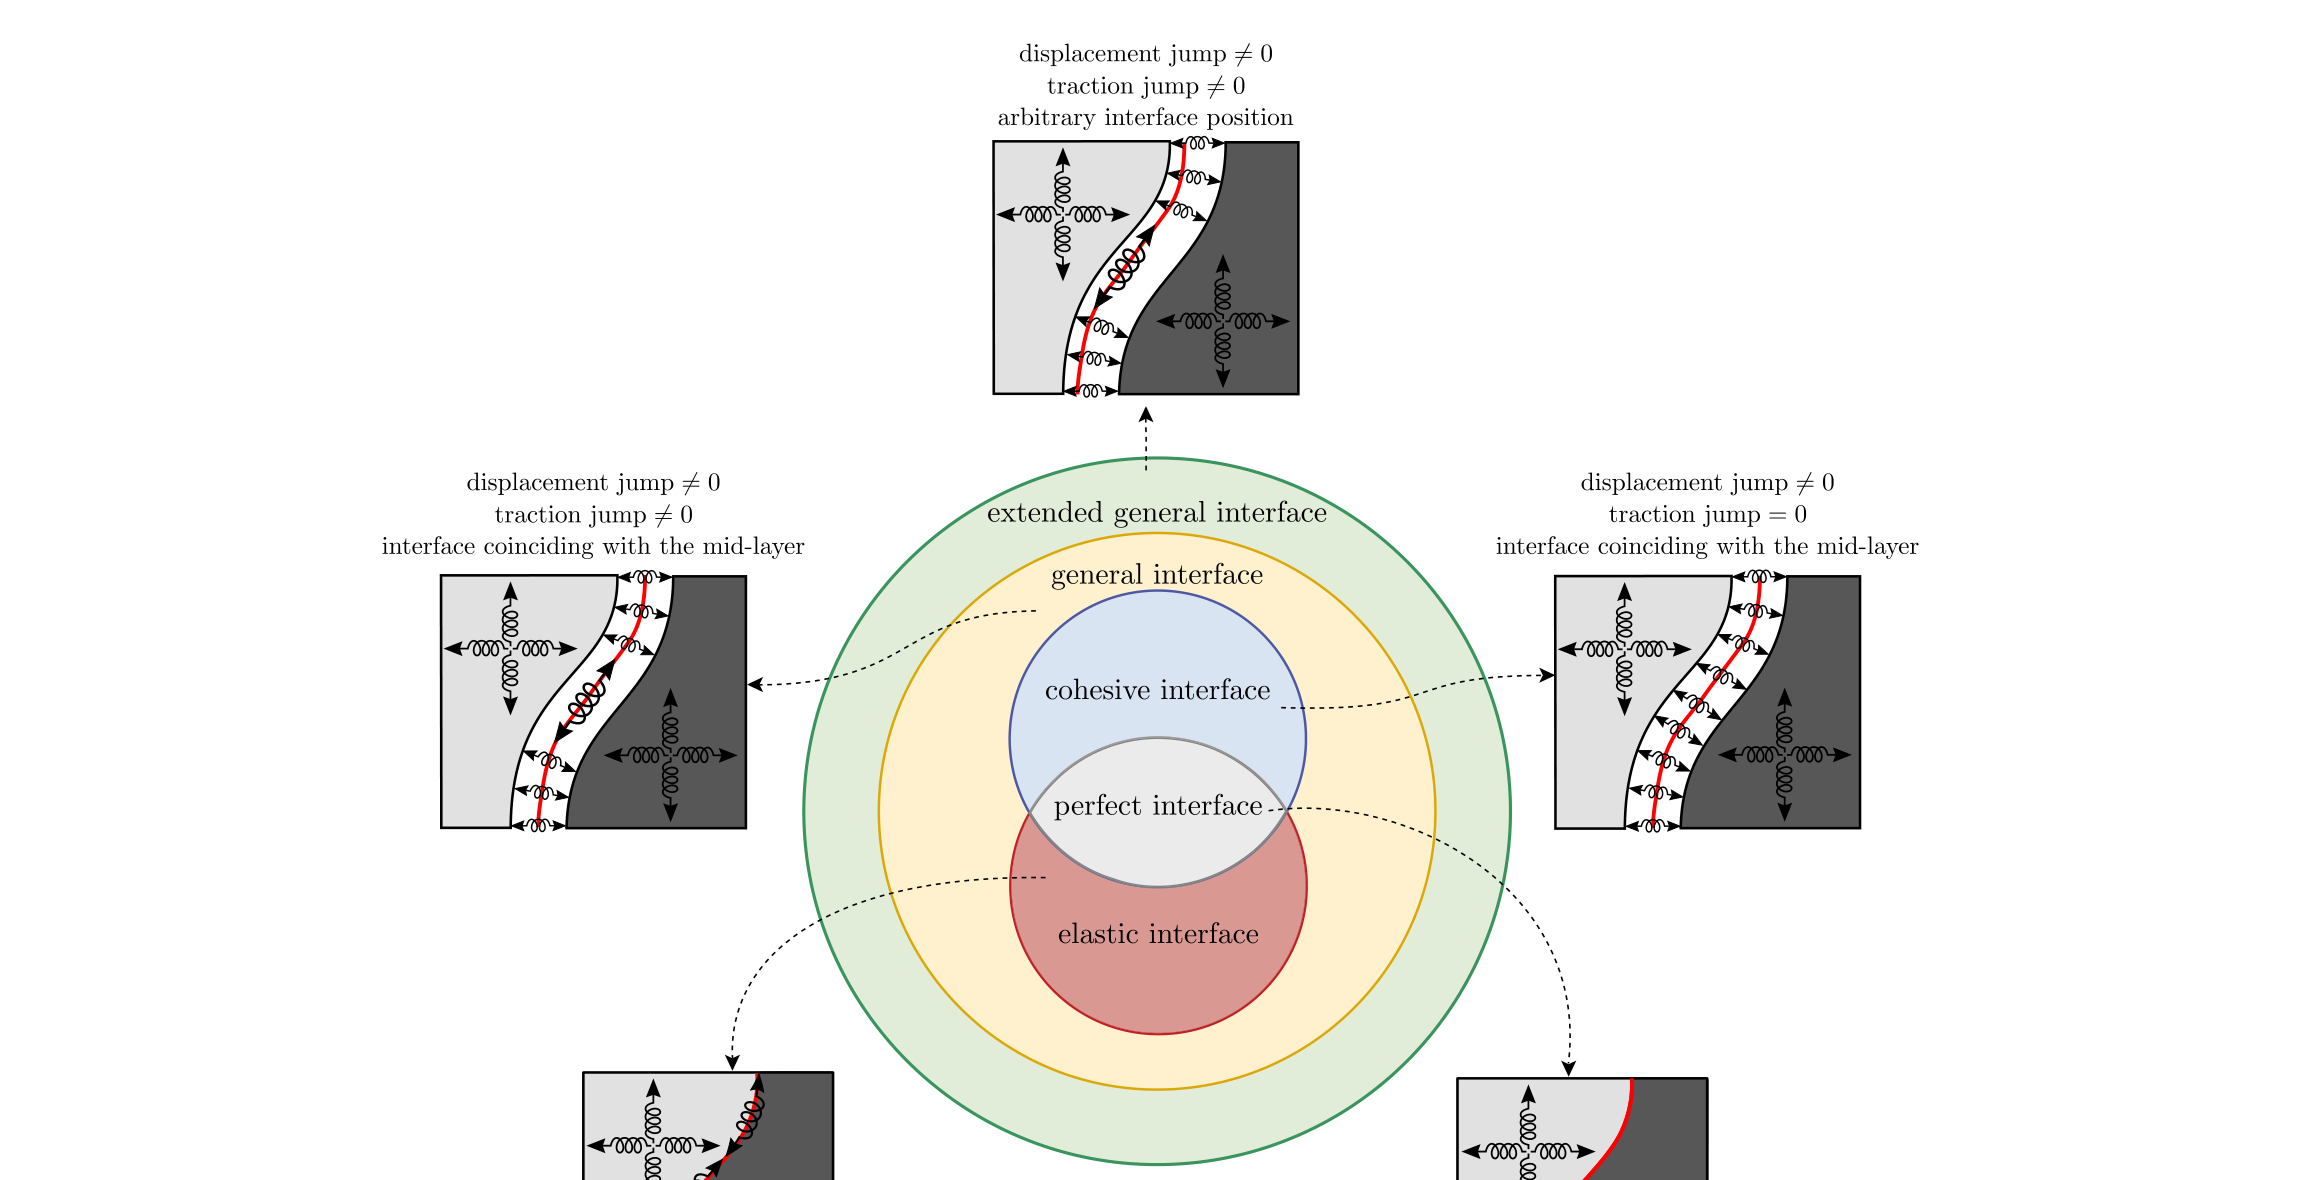
\includegraphics[width=0.95\textwidth]{figures/interface_classification.pdf}
    \fbox{\parbox{0.95\textwidth}{\centering\vspace{1.5cm}
    \textbf{[Insert Figure 1 from Firooz et al. (2021)]}\\[0.5em]
    \small Classification showing: Perfect, Cohesive, Elastic, General, and Extended General Interface models based on displacement jump and traction jump conditions
    \vspace{1.5cm}}}
    \caption{Classification of interface models based on kinematic (displacement) and kinetic (traction) coherence. The extended general interface model encompasses all classical models while additionally allowing arbitrary interface positioning. Adapted from \cite{Firooz2021}.}
    \label{fig:interface_classification}
\end{figure}

\subsection{Imperfect Interface Models}

Relaxing one continuity condition while maintaining the other leads to two canonical imperfect interface models:

\paragraph{Cohesive (Spring-Layer) Interface:}
Traction remains continuous while displacement may jump in proportion to the interface traction \cite{Hashin1991, Needleman1987}:
%
\begin{equation}
    \jump{\bs{t}} = \bs{0}, \quad \mean{\bs{t}} = \bar{k} \jump{\bs{u}}
    \label{eq:cohesive_interface}
\end{equation}
%
where $\mean{\cdot}$ denotes the average across the interface and $\bar{k}$ is the interface stiffness. This model represents compliant interphases---soft coatings, adhesive layers, or degraded bonds.

\paragraph{Elastic (Membrane) Interface:}
Displacement remains continuous while traction may jump due to surface stresses \cite{Gurtin1975}:
%
\begin{equation}
    \jump{\bs{u}} = \bs{0}, \quad \jump{\bs{t}} = -\nabla_{\mathcal{I}} \cdot \bar{\bs{\sigma}}
    \label{eq:elastic_interface}
\end{equation}
%
where $\bar{\bs{\sigma}}$ is the interface stress and $\nabla_{\mathcal{I}}$ is the surface divergence operator. Based on Gurtin-Murdoch surface elasticity theory \cite{Gurtin1975, Gurtin1978}, this model captures stiff interphases that resist tangential deformation, characterized by interface elastic modulus $\bar{\mu}$.

\subsection{General Interface Model}

Real interphases often exhibit characteristics of both soft and hard behavior simultaneously. Hashin \cite{Hashin2002} and Benveniste and Miloh \cite{Benveniste2001} unified the cohesive and elastic models into a \textit{general interface model} (GIM) admitting both displacement and traction jumps:
%
\begin{align}
    \mean{\bs{t}} &= \bar{k} \jump{\bs{u}} \label{eq:gim_cohesive_intro} \\
    \jump{\bs{t}} &= -\nabla_{\mathcal{I}} \cdot \bar{\bs{\sigma}} \label{eq:gim_elastic_intro}
\end{align}
%
The cohesive and elastic models emerge as limiting cases: $\bar{k} \to \infty$ with $\bar{\mu} = 0$ recovers the perfect interface; finite $\bar{k}$ with $\bar{\mu} = 0$ gives the cohesive interface; $\bar{k} \to \infty$ with finite $\bar{\mu}$ produces the elastic interface.

These phenomenological models find rigorous justification through asymptotic analysis. Lebon and Rizzoni \cite{Lebon2010, Lebon2011} showed that as interphase thickness $\varepsilon \to 0$, the emergent interface law depends on how stiffness scales with thickness: soft scaling ($\mathbb{C} \sim \varepsilon$) yields the cohesive model, while stiff scaling ($\mathbb{C} \sim \varepsilon^{-1}$) produces the elastic model.

\subsection{Extended General Interface Model}

A crucial limitation of the classical GIM is the implicit assumption that the interface coincides with the geometric mid-plane of the interphase---problematic for graded or asymmetric interphases. Firooz et al. \cite{Firooz2019, Firooz2021} addressed this by introducing the \textit{Extended General Interface Model} (EGIM), which allows the interface to occupy any position within the original interphase through a weighted average operator:
%
\begin{equation}
    \mean{\phi}_{\bar{\alpha}} := \bar{\alpha} \phi^+ + (1 - \bar{\alpha}) \phi^-
    \label{eq:weighted_average_intro}
\end{equation}
%
where $\bar{\alpha} \in [0, 1]$ is the interface position parameter. Setting $\bar{\alpha} = 0.5$ recovers the standard mid-plane assumption, while $\bar{\alpha} = 0$ or $1$ places the interface at the inclusion or matrix boundary, respectively.

The complete EGIM is characterized by four independent parameters:
%
\begin{itemize}
    \item $\bar{k}$ --- orthogonal stiffness (resistance to normal separation)
    \item $\bar{\lambda}$ --- interface Lam\'{e} parameter
    \item $\bar{\mu}$ --- interface shear modulus (resistance to tangential deformation)
    \item $\bar{\alpha}$ --- position parameter (location within the interphase)
\end{itemize}
%
This extended model can recover all classical interface types while additionally capturing graded interphases through appropriate choice of $\bar{\alpha}$ \cite{Firooz2021}.

% -------------------------------------------------------------------
\section{The Research Gap: Parameter Identification}
% -------------------------------------------------------------------

The theoretical framework described above provides a coherent path from finite-thickness interphases to computationally efficient interface models. However, a critical gap remains in practical application: the interface parameters ($\bar{k}$, $\bar{\mu}$, $\bar{\alpha}$) are phenomenological quantities that cannot be directly measured or straightforwardly derived from known interphase properties.

Consider a concrete example: given a CFRP system with a sizing layer of known thickness $h$ and elastic moduli ($\lambda_{\text{sizing}}$, $\mu_{\text{sizing}}$), what interface stiffness $\bar{k}$ produces the same effective composite response? The answer is not obvious, and several complicating factors arise:

\paragraph{Non-uniqueness:} Different combinations of interface parameters can yield identical macroscopic responses. For instance, increasing $\bar{k}$ while simultaneously adjusting $\bar{\alpha}$ may leave the effective bulk modulus unchanged \cite{Firooz2021}.

\paragraph{Coupled Effects:} The interface parameters influence multiple effective properties simultaneously. The stiffness $\bar{k}$ affects both bulk and shear moduli, making independent identification from single loading cases difficult.

\paragraph{Graded Properties:} Real interphases rarely exhibit uniform properties. Sizing agents create cross-linking density gradients \cite{Wu2019}, diffusion processes generate compositional profiles, and damage accumulation produces spatially varying stiffness. Mapping such complexity onto equivalent interface parameters requires systematic methodology.


% ===================================================================
% NEW SUBSECTION TO ADD IN SECTION 1.5 (after "Graded Properties" paragraph)
% Place this BEFORE Section 1.6 "Bridging the Gap: A Data-Driven Approach"
% ===================================================================

\subsection{Approaches to Parameter Identification}
\label{subsec:approaches_param_id}

Two fundamentally different strategies exist for determining interface parameters from interphase descriptions: asymptotic derivation and direct parametric identification. Understanding their limitations motivates the data-driven approach adopted in this thesis.

\paragraph{Asymptotic Approach.}
The most rigorous route to interface parameters proceeds through asymptotic analysis, treating the interphase thickness $\varepsilon$ as a small parameter and examining the limiting behavior as $\varepsilon \to 0$. Pioneered by B\"{o}vik \cite{Bovik1994} and systematically developed by Benveniste \cite{Benveniste2006}, this methodology expands the fields within the interphase using Taylor series about the mid-surface, then enforces continuity conditions at the boundaries. The resulting transmission conditions across the zero-thickness interface emerge naturally from this limiting process.

The key insight from asymptotic analysis is that the \textit{scaling} of interphase stiffness with thickness determines the interface type. When the Lam\'{e} parameters scale as $\lambda^\varepsilon = \varepsilon\bar{\lambda}$ and $\mu^\varepsilon = \varepsilon\bar{\mu}$ (soft interphase), the analysis yields a cohesive-type interface with stiffness $\bar{k} = \mu/h$. Conversely, when stiffness scales inversely with thickness (stiff interphase), a membrane-type interface emerges with surface elastic parameters \cite{Lebon2010, Lebon2011}. Serpilli et al.\ \cite{Serpilli2019} extended this framework to multiphysics problems, while Baranova and Mogilevskaya \cite{Baranova2022} provided a comprehensive comparison of related methodologies.

The elegance of asymptotic methods lies in deriving interface parameters directly from known interphase properties---no curve fitting or optimization is required. However, this approach presupposes complete knowledge of the interphase: its thickness, elastic moduli, and how these scale with geometric parameters. In practice, interphase properties are often uncertain, spatially graded, or only partially characterized through indirect measurements. Moreover, asymptotic analysis assumes specific scaling regimes; real interphases may exhibit mixed soft-hard behavior that does not fit neatly into these categories.

\paragraph{Direct Parametric Identification.}
An alternative strategy attempts to identify interface parameters by requiring that the interface model reproduce the same effective composite response as the interphase model. Given concentration tensors $\mathbb{T}^{\text{eq}}_{\text{interphase}}$ and $\mathbb{H}^{\text{eq}}_{\text{interphase}}$ computed from a multi-coated inclusion analysis, one seeks interface parameters $(\bar{k}, \bar{\lambda}, \bar{\mu}, \bar{\alpha})$ such that:
%
\begin{equation}
    \mathbb{T}^{\text{eq}}_{\text{interface}}(\bar{k}, \bar{\lambda}, \bar{\mu}, \bar{\alpha}) = \mathbb{T}^{\text{eq}}_{\text{interphase}}
    \label{eq:matching_condition}
\end{equation}

This matching condition, while conceptually appealing, leads to a fundamental mathematical difficulty. For isotropic particle composites, the concentration tensors provide only two independent scalar equations---one from the bulk response ($T_\kappa^{\text{eq}}$) and one from the shear response ($T_\mu^{\text{eq}}$). Yet the Extended General Interface Model contains three to four unknown parameters: orthogonal stiffness $\bar{k}$, interface Lam\'{e} parameters $\bar{\lambda}$ and $\bar{\mu}$, and position parameter $\bar{\alpha}$.

The system is therefore \textit{underdetermined}: more unknowns than equations. Even for fiber composites, where three independent loading modes (bulk, transverse shear, axial shear) provide additional constraints, the position parameter $\bar{\alpha}$ introduces coupling that prevents straightforward inversion. Physically, this underdetermination reflects the fact that different interface mechanisms can produce identical macroscopic responses---a stiffer interface positioned closer to the matrix may yield the same effective modulus as a more compliant interface closer to the fiber \cite{Firooz2021}.

Attempts to close the system through simplifying assumptions---such as fixing $\bar{\alpha} = 0.5$ (mid-plane position) or assuming $\bar{\lambda} = \bar{\mu}$---sacrifice generality and may introduce systematic errors for graded or asymmetric interphases. The direct parametric approach, despite its intuitive appeal, cannot provide a unique and general solution to the parameter identification problem.

\paragraph{Motivation for Data-Driven Methods.}
The limitations of both approaches point toward an alternative strategy. Asymptotic methods require detailed interphase characterization that may be unavailable; direct matching yields underdetermined systems without unique solutions. What is needed is a framework that can:
%
\begin{enumerate}
    \item Learn the complex, potentially non-unique mapping between mechanical response and interface parameters from data
    \item Generalize across different material systems and interphase configurations
    \item Provide rapid predictions once trained, enabling efficient material design
\end{enumerate}
%
Neural networks are naturally suited to such inverse problems. By training on a large database of forward simulations---where interface parameters are varied and the resulting concentration tensors computed---the network learns to navigate the parameter space and identify physically meaningful solutions even when the analytical inverse does not exist. This data-driven approach forms the core of the methodology developed in this thesis.




% -------------------------------------------------------------------
\section{Bridging the Gap: A Data-Driven Approach}
% -------------------------------------------------------------------

The limitations outlined above---underdetermined inverse problems, non-unique parameter mappings, and incomplete interphase characterisation---suggest that purely analytical routes to parameter identification have inherent constraints. This thesis develops a computational framework that combines analytical homogenization with neural networks to address these challenges through two complementary strategies.

\paragraph{Gap Analysis of the Extended Interface Model.}
A natural question is whether the Extended General Interface Model, with suitably chosen parameters, can reproduce the multi-coated interphase predictions. We investigate this systematically by allowing a global optimiser to find the best-fit interface parameters for each configuration independently---giving the interface model every possible advantage. This analysis reveals whether the discrepancy between the two models is parametric (fixable by better parameter choices) or structural (inherent to the zero-thickness assumption).

\paragraph{Inverse Parameter Identification via Physics-Informed Neural Networks.}
Where the interface model is applicable, we develop a physics-informed neural network (PINN) that directly identifies interface parameters from target mechanical response. Unlike conventional inverse optimisation, the PINN embeds the governing homogenization equations into its loss function, enabling parameter identification that respects physical constraints without requiring repeated forward solves. We apply the same inverse network to both CSA and CCA geometries---the CSA case tests the method where the interface model is structurally adequate, while the CCA case provides independent confirmation of the gap analysis.

The choice of neural networks over alternative methods---such as Gaussian process regression \cite{Rasmussen2006} or polynomial chaos expansions \cite{Xiu2002}---is motivated by the problem characteristics. The input space is seven- to eight-dimensional (effective moduli, elastic constants, and volume fraction), the input-output mapping is highly nonlinear, and the material properties span several orders of magnitude. Gaussian processes scale cubically with training set size, making them impractical for the $200\,000$-sample datasets used here \cite{Liu2020}. Polynomial expansions struggle with the strong nonlinearities and high dimensionality of the parameter space. Neural networks handle both challenges naturally through their universal approximation capability and efficient mini-batch training \cite{Hornik1989}.

% -------------------------------------------------------------------
\section{Objectives}
% -------------------------------------------------------------------

The primary objective of this thesis is to investigate the relationship between finite-thickness interphase models and zero-thickness interface models in composite homogenization, and to develop neural network approaches where analytical methods reach their limits. Specifically, the research aims to:

\begin{enumerate}
    \item \textbf{Implement and Verify the Multi-Coated Interphase Model:} Develop and validate implementations of the three-layered interphase boundary value problems for both fibre-reinforced (CCA) and particle-reinforced (CSA) composites, establishing a trusted reference solution through consistency checks and limiting-case verification.

    \item \textbf{Quantify the Representational Limits of the Extended Interface Model:} Systematically compare the Extended General Interface Model against the three-layered interphase predictions, using both isotropic (4-parameter) and anisotropic (7-parameter) formulations with globally optimised parameters, to determine whether discrepancies are parametric or structural in nature.

    \item \textbf{Develop an Inverse PINN for Parameter Identification:} Construct a physics-informed neural network that identifies interface parameters from target mechanical response, embedding the homogenization equations directly into the training process. Apply this to the CSA geometry where the interface model is structurally adequate.

    \item \textbf{Confirm the Gap via CCA Inverse PINN:} Apply the same inverse PINN to CCA composites to verify independently that the interface--interphase discrepancy is structural rather than an artefact of the optimisation procedure.

    \item \textbf{Synthesise the Findings:} Compare all methods---analytical optimisation, inverse PINN for CSA, and inverse PINN for CCA---to establish when the Extended Interface model is applicable and when it is not, defining clear scope boundaries for different composite geometries.
\end{enumerate}
\newpage
% -------------------------------------------------------------------
\section{Structure of the Thesis}
% -------------------------------------------------------------------

This work is structured as follows:

\textbf{Chapter~\ref{ch:theory}} presents the theoretical foundations. It begins with the governing equations of continuum mechanics and homogenization---balance laws, the Hill-Mandel condition, and the Eshelby inclusion problem. The coordinate transformation machinery for cylindrical and spherical geometries is then established. The multi-coated inclusion model for interphase analysis is developed, the concentration tensor structures are derived, and the interface models from perfect to extended general are formulated. The chapter concludes with the interface-enhanced Mori-Tanaka homogenization framework.

\textbf{Chapter~\ref{ch:methodology}} develops the methodology. The boundary value problems for the multi-layered interphase model and the interface-enhanced Mori-Tanaka model are derived for fibre-reinforced (CCA) and particle-reinforced (CSA) composites. The neural network architecture for inverse parameter identification is presented, along with training procedures and data generation.

\textbf{Chapter~\ref{ch:results}} presents the results and discussion. The three-layered interphase model is first verified through consistency checks and limiting cases. The representational limits of the Extended Interface Model are quantified through systematic gap analysis with worked numerical examples. Inverse PINNs for both CSA and CCA geometries are demonstrated, with the CCA case providing independent confirmation of the gap. The chapter concludes with a discussion of the findings and practical recommendations.

\textbf{Chapter~\ref{ch:conclusion}} summarises the contributions, discusses limitations of the current framework, and outlines directions for future research.


% -----------------------------------------------------------------

% ===================================================================
%   CHAPTER 2: THEORETICAL FOUNDATIONS 
%   Aligned with Methodology using Extended Mori-Tanaka Framework
% ===================================================================
\chapter{Theoretical Foundations}
\label{ch:theory}

This chapter presents the two theoretical models that form the basis of the present work. We begin with a brief set of preliminaries---the Representative Volume Element, balance of momentum, constitutive relations, and the Hill-Mandel and Eshelby frameworks---that both models build upon. Section~\ref{sec:interphase_model} then develops the three-layered interphase model, where a graded interphase region is discretised into coating layers with piecewise-constant properties. We define the volume fractions, concentration tensors, and homogenization formulas for both fibre-reinforced (2D, CCA) and particle-reinforced (3D, CSA) composites. Section~\ref{sec:interface_model} presents the alternative approach: the Extended General Interface Model (EGIM), which replaces the finite-thickness interphase with a zero-thickness surface governed by interface constitutive laws. We develop the interface kinematics, model hierarchy, modified averaging relations, and the Mori-Tanaka homogenization with interface effects. The boundary value problems that determine the concentration tensor components for both models are derived in Chapter~\ref{ch:methodology}.

% ===================================================================
\section{Preliminaries}
\label{sec:preliminaries}
% ===================================================================

Before developing the two models, we establish the continuum mechanics framework that underpins homogenization.

% -------------------------------------------------------------------
\subsection{Representative Volume Element}
\label{subsec:rve}
% -------------------------------------------------------------------

Homogenization relies on the concept of a Representative Volume Element (RVE)---a material domain $\mathcal{V}$ large enough to capture the statistical character of the microstructure yet small enough that macroscopic fields remain approximately uniform across it \cite{Hill1963}. This separation of scales,
%
\begin{equation}
    \ell_{\text{micro}} \;\ll\; \ell_{\text{RVE}} \;\ll\; \ell_{\text{macro}},
    \label{eq:scale_separation}
\end{equation}
%
where $\ell_{\text{micro}}$ is the characteristic inclusion size (fibre radius or particle diameter), $\ell_{\text{RVE}}$ the RVE dimension, and $\ell_{\text{macro}}$ the structural length scale, is the basic requirement for any mean-field homogenization scheme. When this condition holds, the heterogeneous material can be replaced by an equivalent homogeneous medium whose effective stiffness ${}^{\mathrm{M}}\hspace{-1pt}\mathbb{C}$ relates macroscopic stress and strain.

For composite cylinder and composite sphere assemblages used in this work, the RVE is a single coated inclusion surrounded by matrix material. Hashin \cite{Hashin1964} showed that assemblages of such unit cells, packed to fill all available space, yield exact effective properties. This is a stronger result than approximate mean-field estimates, and it provides the benchmark against which our numerical implementations are verified in Chapter~\ref{ch:results}.

% -------------------------------------------------------------------
\subsection{Balance of Linear Momentum}
\label{subsec:balance_equations}
% -------------------------------------------------------------------

Within the RVE, each phase satisfies the static balance of linear momentum in the absence of body forces:
%
\begin{equation}
    \nabla \cdot \bs{\sigma} = \bs{0}, \quad \bs{x} \in \mathcal{B}
    \label{eq:bulk_equilibrium}
\end{equation}
%
where $\mathcal{B}$ denotes the bulk domain (all phases).

% -------------------------------------------------------------------
\subsection{Constitutive Relations}
\label{subsec:constitutive_relations}
% -------------------------------------------------------------------

Both models in this thesis assume linear elastic, isotropic phase materials. The strain and stress tensors in Voigt notation are:
%
\begin{equation}
    \bs{\varepsilon} =
    \begin{bmatrix}
        \varepsilon_{11} & \varepsilon_{22} & \varepsilon_{33} & 2\varepsilon_{12} & 2\varepsilon_{13} & 2\varepsilon_{23}
    \end{bmatrix}^T
    \label{eq:strain_voigt}
\end{equation}
%
\begin{equation}
    \bs{\sigma} =
    \begin{bmatrix}
        \sigma_{11} & \sigma_{22} & \sigma_{33} & \sigma_{12} & \sigma_{13} & \sigma_{23}
    \end{bmatrix}^T
    \label{eq:stress_voigt}
\end{equation}

For isotropic phases, the stiffness tensor takes the form:
%
\begin{equation}
    \mathbb{L} = \lambda \, \bs{I} \otimes \bs{I} + 2\mu \, \mathbb{I}^{\text{sym}}
    \label{eq:isotropic_stiffness}
\end{equation}
%
where $\lambda$ and $\mu$ are the Lam\'{e} parameters. In matrix form:
%
\begin{equation}
    \mathbb{L} =
    \begin{bmatrix}
        \lambda + 2\mu & \lambda & \lambda & 0 & 0 & 0 \\
        \lambda & \lambda + 2\mu & \lambda & 0 & 0 & 0 \\
        \lambda & \lambda & \lambda + 2\mu & 0 & 0 & 0 \\
        0 & 0 & 0 & \mu & 0 & 0 \\
        0 & 0 & 0 & 0 & \mu & 0 \\
        0 & 0 & 0 & 0 & 0 & \mu
    \end{bmatrix}
    \label{eq:stiffness_matrix}
\end{equation}

The plane-strain bulk modulus is $\kappa = \lambda + \mu$ and the 3D bulk modulus is $K = \lambda + \frac{2}{3}\mu$.

% -------------------------------------------------------------------
\subsection{Hill-Mandel Condition}
\label{subsec:hill_mandel}
% -------------------------------------------------------------------

The Hill-Mandel condition ensures energy consistency between the micro and macro scales. It requires that the macroscopic stress power equals the volume average of the microscopic stress power over the RVE. For a body $\mathcal{B}$ with boundary $\partial\mathcal{B}$ subject to linear displacement boundary conditions $\bs{u} = {}^{\mathrm{M}}\hspace{-1pt}\bs{\varepsilon} \cdot \bs{x}$, the macroscopic strain and stress are defined as boundary integrals \cite{Firooz2022}:
%
\begin{align}
    {}^{\mathrm{M}}\hspace{-1pt}\bs{\varepsilon} &= \frac{1}{\mathcal{V}} \int_{\partial\mathcal{B}} \frac{1}{2} \left(\bs{u} \otimes \bs{n} + \bs{n} \otimes \bs{u}\right) \dd A \label{eq:macro_strain_boundary}\\[4pt]
    {}^{\mathrm{M}}\hspace{-1pt}\bs{\sigma} &= \frac{1}{\mathcal{V}} \int_{\partial\mathcal{B}} \bs{t} \otimes \bs{x} \;\dd A \label{eq:macro_stress_boundary}
\end{align}
%
where $\mathcal{V}$ is the RVE volume, $\bs{n}$ the outward unit normal on $\partial\mathcal{B}$, and $\bs{t} = \bs{\sigma} \cdot \bs{n}$ the surface traction.

The Hill-Mandel condition then requires:
%
\begin{equation}
    \int_{\partial\mathcal{B}} \left[\delta\bs{u} - \delta {}^{\mathrm{M}}\hspace{-1pt}\bs{\varepsilon} \cdot \bs{x}\right] \cdot \left[\bs{t} - {}^{\mathrm{M}}\hspace{-1pt}\bs{\sigma} \cdot \bs{n}\right] \dd A = 0
    \label{eq:hill_mandel}
\end{equation}

This is satisfied by linear displacement (Dirichlet) boundary conditions, uniform traction (Neumann) boundary conditions, or periodic boundary conditions \cite{Hill1963}. In the Mori-Tanaka framework used throughout this thesis, we adopt linear displacement boundary conditions: $\bs{u} = \bs{\varepsilon}^{(0)} \cdot \bs{x}$ at infinity.

% -------------------------------------------------------------------
\subsection{Eshelby Inclusion Problem and the Mori-Tanaka Assumption}
\label{subsec:eshelby_problem}
% -------------------------------------------------------------------

The Eshelby inclusion problem \cite{Eshelby1957} considers a single ellipsoidal inhomogeneity with stiffness $\mathbb{L}^{(1)}$ embedded in an infinite matrix with stiffness $\mathbb{L}^{(0)}$, subject to a uniform far-field strain $\bs{\varepsilon}^{(0)}$. Eshelby's fundamental result is that the strain inside the inhomogeneity is uniform, and the \textit{dilute} strain concentration tensor $\mathbb{T}_{\text{dil}}$ satisfies:
%
\begin{equation}
    \bs{\varepsilon}^{(1)} = \mathbb{T}_{\text{dil}} : \bs{\varepsilon}^{(0)}, \quad
    \mathbb{T}_{\text{dil}} = \left[\mathbb{I} + \mathbb{S} : \left(\mathbb{L}^{(0)}\right)^{-1} : \left(\mathbb{L}^{(1)} - \mathbb{L}^{(0)}\right)\right]^{-1}
    \label{eq:eshelby_dilute}
\end{equation}
%
where $\mathbb{S}$ is the Eshelby tensor, which depends only on the inclusion shape and the matrix Poisson's ratio. For spherical inclusions and cylindrical fibres, $\mathbb{S}$ has well-known closed-form expressions \cite{Eshelby1957}.

The Mori-Tanaka method \cite{Mori1973, Benveniste1987} extends this dilute result to finite inclusion volume fractions by a mean-field assumption: each inclusion experiences the \textit{average matrix strain} $\bs{\varepsilon}^{(2)}$ (rather than the macroscopic strain) as its far-field condition. The effective stiffness then follows from the dilute tensors and volume fractions.

For composites with imperfect interfaces, the classical Eshelby formula~\eqref{eq:eshelby_dilute} no longer applies directly, because the interface conditions modify the stress and displacement fields around the inclusion. In this case, the concentration tensors are computed by solving boundary value problems that incorporate the specific interface constitutive law---a procedure detailed in Chapter~\ref{ch:methodology}.

% ===================================================================
\section{Three-Layered Interphase Model}
\label{sec:interphase_model}
% ===================================================================

In many composite systems, the transition from inclusion to matrix is not abrupt but occurs through a graded interphase region with spatially varying properties. The three-layered interphase model handles this by discretising the interphase into $N$ coating layers, each with piecewise-constant material properties. An inhomogeneity (core) with stiffness $\mathbb{L}_h$ is surrounded by coating layers with stiffnesses $\mathbb{L}_1, \mathbb{L}_2, \ldots, \mathbb{L}_N$, all embedded in an infinite matrix with stiffness $\mathbb{L}_0$ subject to a uniform far-field strain. In the present work, we use $N=3$ coating layers, which convergence studies show is sufficient for most engineering interphase profiles.

% -------------------------------------------------------------------
\subsection{Average Fields and Volume Fractions}
\label{subsec:average_fields}
% -------------------------------------------------------------------

For homogenization, we define the average strain and stress in each phase $i$:
%
\begin{equation}
    \bs{\varepsilon}^{(i)} = \frac{1}{V_i} \int_{\Omega_i} \bs{\varepsilon}(\bs{x}) \, dV, \quad
    \bs{\sigma}^{(i)} = \frac{1}{V_i} \int_{\Omega_i} \bs{\sigma}(\bs{x}) \, dV
    \label{eq:average_fields}
\end{equation}
%
for $i = h, 1, 2, \ldots, N, 0$.

\label{subsec:volume_fractions}
The volume fractions characterise the relative sizes of the phases within the equivalent inhomogeneity:
%
\begin{equation}
    c_h = \frac{V_h}{V_h + \sum_{r=1}^{N} V_r}, \quad
    c_m = \frac{V_m}{V_h + \sum_{r=1}^{N} V_r}, \quad
    \phi_m = \frac{V_h + \sum_{r=1}^{m-1} V_r}{V_h + \sum_{r=1}^{m} V_r}
    \label{eq:volume_fractions_general}
\end{equation}
%
where $V_h$ is the core volume and $V_m$ the volume of coating layer $m$. These can be expressed recursively:
%
\begin{align}
    c_N &= 1 - \phi_N \nonumber\\
    c_{N-1} &= \phi_N - \phi_N \phi_{N-1} \nonumber\\
    c_{N-2} &= \phi_N \phi_{N-1} - \phi_N \phi_{N-1} \phi_{N-2} \nonumber\\
    &\vdots \nonumber\\
    c_1 &= \phi_N \phi_{N-1} \cdots \phi_2 - \phi_N \phi_{N-1} \cdots \phi_2 \phi_1 \nonumber\\
    c_h &= \phi_N \phi_{N-1} \cdots \phi_2 \phi_1
    \label{eq:volume_fractions_recursive}
\end{align}

The geometric formulae differ for the two composite types. For \textbf{coated cylindrical fibres} (2D, CCA geometry):
%
\begin{equation}
    c_h = \frac{r_1^2}{r_{N+1}^2}, \quad c_m = \frac{r_{m+1}^2 - r_m^2}{r_{N+1}^2}, \quad \phi_m = \left(\frac{r_m}{r_{m+1}}\right)^2
    \label{eq:volume_fractions_cylindrical}
\end{equation}

For \textbf{coated spherical particles} (3D, CSA geometry):
%
\begin{equation}
    c_h = \frac{r_1^3}{r_{N+1}^3}, \quad c_m = \frac{r_{m+1}^3 - r_m^3}{r_{N+1}^3}, \quad \phi_m = \left(\frac{r_m}{r_{m+1}}\right)^3
    \label{eq:volume_fractions_spherical}
\end{equation}
%
where $r_1$ is the core radius and $r_m$ denotes the outer radius of coating layer $m-1$ (inner radius of layer $m$).

% -------------------------------------------------------------------
\subsection{Model Assumptions}
\label{subsec:interphase_assumptions}
% -------------------------------------------------------------------

The multi-coated inclusion model rests on the following assumptions:

\begin{enumerate}
    \item \textbf{Linear elasticity} in all phases---the core, each coating layer, and the matrix obey Hooke's law with small deformations.
    \item \textbf{Isotropic phase materials}: each phase is characterised by two Lam\'{e} parameters $(\lambda^{(q)}, \mu^{(q)})$, constant within each phase.
    \item \textbf{Perfect bonding} between adjacent layers---displacement and traction are continuous across every internal boundary $\partial\Omega_m$.
    \item \textbf{Piecewise-constant property approximation}: a continuously graded interphase is discretised into $N$ layers of uniform properties.
    \item \textbf{Dilute embedding}: the multicoated inclusion sits in an infinite matrix subject to a uniform far-field strain $\bs{\varepsilon}^{(0)}$ (Eshelby problem setting).
    \item \textbf{Concentration tensor extraction}: the tensors $\mathbb{T}^{(q)}$ and $\mathbb{H}^{(q)}$ are obtained from volume-averaged strain and stress fields over each phase, computed from the BVP solutions derived in Chapter~\ref{ch:methodology}.
\end{enumerate}

% -------------------------------------------------------------------
\subsection{Coordinate Transformations}
\label{sec:coordinate_transform}
% -------------------------------------------------------------------

The boundary value problems are formulated in curvilinear coordinates---cylindrical $(r, \theta, z)$ for fibres and spherical $(r, \theta, \phi)$ for particles. Since the concentration tensors are expressed in Voigt notation with respect to Cartesian axes, we need transformation matrices that convert between coordinate systems.

\subsubsection{Rotation Matrix}
\label{subsec:rotation_matrix}

A second-order tensor rotator $\bs{R}$ maps components from the global Cartesian frame $(x_1, x_2, x_3)$ to a local frame:
%
\begin{equation}
    \bs{R} =
    \begin{bmatrix}
        R_{11} & R_{12} & R_{13} \\
        R_{21} & R_{22} & R_{23} \\
        R_{31} & R_{32} & R_{33}
    \end{bmatrix}
    \label{eq:rotation_matrix}
\end{equation}

For \textbf{cylindrical coordinates} (2D, CCA) with the fibre axis along $z$:
%
\begin{equation}
    \bs{R}_{\text{cyl}} =
    \begin{bmatrix}
        \cos\theta & -\sin\theta & 0 \\
        \sin\theta & \cos\theta & 0 \\
        0 & 0 & 1
    \end{bmatrix}
    \label{eq:R_cylindrical}
\end{equation}

For \textbf{spherical coordinates} (3D, CSA):
%
\begin{equation}
    \bs{R}_{\text{sph}} =
    \begin{bmatrix}
        \sin\theta\cos\phi & \cos\theta\cos\phi & -\sin\phi \\
        \sin\theta\sin\phi & \cos\theta\sin\phi & \cos\phi \\
        \cos\theta & -\sin\theta & 0
    \end{bmatrix}
    \label{eq:R_spherical}
\end{equation}

\subsubsection{Voigt Transformation Matrices}
\label{subsec:Q_matrices}

The rotator $\bs{R}$ is represented in Voigt notation by two $6 \times 6$ matrices $\bs{Q}_\varepsilon$ and $\bs{Q}_\sigma$ for transforming strains and stresses, respectively. The distinction arises from the engineering shear strain convention: strain components carry a factor of 2 (e.g., $\gamma_{12} = 2\varepsilon_{12}$), while stress components do not.

The strain transformation matrix $\bs{Q}_\varepsilon$ ($\bs{\varepsilon}' = \bs{Q}_\varepsilon \cdot \bs{\varepsilon}$):
%
\begin{equation}
    \bs{Q}_\varepsilon =
    \begin{bmatrix}
        R_{11}^2 & R_{21}^2 & R_{31}^2 & R_{11}R_{21} & R_{11}R_{31} & R_{21}R_{31} \\
        R_{12}^2 & R_{22}^2 & R_{32}^2 & R_{12}R_{22} & R_{12}R_{32} & R_{22}R_{32} \\
        R_{13}^2 & R_{23}^2 & R_{33}^2 & R_{13}R_{23} & R_{13}R_{33} & R_{23}R_{33} \\
        2R_{11}R_{12} & 2R_{21}R_{22} & 2R_{31}R_{32} & R_{12}R_{21}+R_{11}R_{22} & R_{12}R_{31}+R_{11}R_{32} & R_{22}R_{31}+R_{21}R_{32} \\
        2R_{11}R_{13} & 2R_{21}R_{23} & 2R_{31}R_{33} & R_{13}R_{21}+R_{11}R_{23} & R_{13}R_{31}+R_{11}R_{33} & R_{23}R_{31}+R_{21}R_{33} \\
        2R_{12}R_{13} & 2R_{22}R_{23} & 2R_{32}R_{33} & R_{13}R_{22}+R_{12}R_{23} & R_{13}R_{32}+R_{12}R_{33} & R_{23}R_{32}+R_{22}R_{33}
    \end{bmatrix}
    \label{eq:Q_epsilon}
\end{equation}

The stress transformation matrix $\bs{Q}_\sigma$ ($\bs{\sigma}' = \bs{Q}_\sigma \cdot \bs{\sigma}$):
%
\begin{equation}
    \bs{Q}_\sigma =
    \begin{bmatrix}
        R_{11}^2 & R_{21}^2 & R_{31}^2 & 2R_{11}R_{21} & 2R_{11}R_{31} & 2R_{21}R_{31} \\
        R_{12}^2 & R_{22}^2 & R_{32}^2 & 2R_{12}R_{22} & 2R_{12}R_{32} & 2R_{22}R_{32} \\
        R_{13}^2 & R_{23}^2 & R_{33}^2 & 2R_{13}R_{23} & 2R_{13}R_{33} & 2R_{23}R_{33} \\
        R_{11}R_{12} & R_{21}R_{22} & R_{31}R_{32} & R_{12}R_{21}+R_{11}R_{22} & R_{12}R_{31}+R_{11}R_{32} & R_{22}R_{31}+R_{21}R_{32} \\
        R_{11}R_{13} & R_{21}R_{23} & R_{31}R_{33} & R_{13}R_{21}+R_{11}R_{23} & R_{13}R_{31}+R_{11}R_{33} & R_{23}R_{31}+R_{21}R_{33} \\
        R_{12}R_{13} & R_{22}R_{23} & R_{32}R_{33} & R_{13}R_{22}+R_{12}R_{23} & R_{13}R_{32}+R_{12}R_{33} & R_{23}R_{32}+R_{22}R_{33}
    \end{bmatrix}
    \label{eq:Q_sigma}
\end{equation}

The forward and inverse transformations are:
%
\begin{align}
    \bs{\varepsilon}' &= \bs{Q}_\varepsilon \cdot \bs{\varepsilon}, \quad \bs{\sigma}' = \bs{Q}_\sigma \cdot \bs{\sigma} \label{eq:transform_forward}\\
    \bs{\varepsilon} &= \bs{Q}_\sigma^T \cdot \bs{\varepsilon}', \quad \bs{\sigma} = \bs{Q}_\varepsilon^T \cdot \bs{\sigma}' \label{eq:transform_inverse}
\end{align}

A useful identity is $\bs{Q}_\varepsilon^{-1} = \bs{Q}_\sigma^T$ and $\bs{Q}_\sigma^{-1} = \bs{Q}_\varepsilon^T$, which follows from the invariance of strain energy density $\frac{1}{2}\bs{\sigma}^T \bs{\varepsilon}$ under coordinate rotation.

% -------------------------------------------------------------------
\subsection{Concentration Tensors}
\label{sec:concentration_tensors_theory}
% -------------------------------------------------------------------

The central goal of the multi-coated inclusion analysis is to determine concentration tensors that relate the average fields in each phase to the applied far-field strain $\bs{\varepsilon}^{(0)}$.

\subsubsection{Strain-Type Concentration Tensor}
\label{subsec:strain_concentration}

The strain-type concentration tensor $\mathbb{T}^{(i)}$ satisfies:
%
\begin{equation}
    \bs{\varepsilon}^{(i)} = \mathbb{T}^{(i)} : \bs{\varepsilon}^{(0)}, \quad i = h, 1, 2, \ldots, N
    \label{eq:strain_concentration}
\end{equation}

\subsubsection{Stress-Strain Concentration Tensor}
\label{subsec:stress_concentration}

The stress-strain concentration tensor $\mathbb{H}^{(i)}$ satisfies:
%
\begin{equation}
    \bs{\sigma}^{(i)} = \mathbb{H}^{(i)} : \bs{\varepsilon}^{(0)}, \quad i = h, 1, 2, \ldots, N
    \label{eq:stress_concentration}
\end{equation}

For phases with constant material properties, these tensors are related by:
%
\begin{equation}
    \mathbb{H}^{(i)} = \mathbb{L}^{(i)} : \mathbb{T}^{(i)}
    \label{eq:H_T_relation}
\end{equation}

\subsubsection{Equivalent Inhomogeneity}
\label{subsec:equivalent_inhomogeneity}

To avoid working with a large number of phases, it is advantageous to replace the inhomogeneity and the multiple coatings with a single \textit{equivalent inhomogeneity}. For an arbitrary field $\bs{a}$ (strain or stress type), its value in the equivalent inhomogeneity is:
%
\begin{equation}
    \bs{a}^{\text{eq}} = c_h \bs{a}^{(h)} + \sum_{r=1}^{N} c_r \bs{a}^{(r)}
    \label{eq:equivalent_field}
\end{equation}
%
where the volume fractions satisfy:
%
\begin{equation}
    c_h + \sum_{i=1}^{N} c_i = 1
    \label{eq:volume_constraint}
\end{equation}

The equivalent concentration tensors are then:
%
\begin{align}
    \mathbb{T}^{\text{eq}} &= c_h \mathbb{T}^{(h)} + \sum_{r=1}^{N} c_r \mathbb{T}^{(r)} \label{eq:Teq}\\
    \mathbb{H}^{\text{eq}} &= c_h \mathbb{H}^{(h)} + \sum_{r=1}^{N} c_r \mathbb{H}^{(r)} \label{eq:Heq}
\end{align}

These are volume-weighted averages over all sub-phases. The BVPs that determine the individual phase tensors are derived in Chapter~\ref{ch:methodology}.

\subsubsection{Tensor Structure for Fibre-Reinforced Composites (2D, CCA)}
\label{subsec:tensor_structure_fiber}

For aligned cylindrical fibres, the composite exhibits transverse isotropy. The concentration tensors in Voigt notation take the block-diagonal form:
%
\begin{equation}
    \mathbb{T}^{(q)} =
    \begin{bmatrix}
        T_{\kappa}^{(q)} + \frac{4}{3}T_{44}^{(q)} & T_{\kappa}^{(q)} - \frac{2}{3}T_{44}^{(q)} & T_{13}^{(q)} & 0 & 0 & 0 \\[4pt]
        T_{\kappa}^{(q)} - \frac{2}{3}T_{44}^{(q)} & T_{\kappa}^{(q)} + \frac{4}{3}T_{44}^{(q)} & T_{13}^{(q)} & 0 & 0 & 0 \\[4pt]
        T_{31}^{(q)} & T_{31}^{(q)} & T_{33}^{(q)} & 0 & 0 & 0 \\[4pt]
        0 & 0 & 0 & T_{44}^{(q)} & 0 & 0 \\[4pt]
        0 & 0 & 0 & 0 & T_{55}^{(q)} & 0 \\[4pt]
        0 & 0 & 0 & 0 & 0 & T_{55}^{(q)}
    \end{bmatrix}
    \label{eq:T_fiber_structure}
\end{equation}
%
The upper-left $3 \times 3$ block couples in-plane and axial responses, while $T_{44}^{(q)}$ and $T_{55}^{(q)}$ govern transverse and axial shear. The stress-strain concentration tensor has the corresponding structure:
%
\begin{equation}
    \mathbb{H}^{(q)} =
    \begin{bmatrix}
        H_{11}^{(q)} & H_{11}^{(q)} - 2H_{44}^{(q)} & H_{13}^{(q)} & 0 & 0 & 0 \\[4pt]
        H_{11}^{(q)} - 2H_{44}^{(q)} & H_{11}^{(q)} & H_{13}^{(q)} & 0 & 0 & 0 \\[4pt]
        H_{31}^{(q)} & H_{31}^{(q)} & H_{33}^{(q)} & 0 & 0 & 0 \\[4pt]
        0 & 0 & 0 & H_{44}^{(q)} & 0 & 0 \\[4pt]
        0 & 0 & 0 & 0 & H_{55}^{(q)} & 0 \\[4pt]
        0 & 0 & 0 & 0 & 0 & H_{55}^{(q)}
    \end{bmatrix}
    \label{eq:H_fiber_structure}
\end{equation}

Six independent components are needed: $T_{\kappa}^{(q)}$, $T_{44}^{(q)}$, $T_{55}^{(q)}$ for $\mathbb{T}$, and $H_{11}^{(q)}$, $H_{44}^{(q)}$, $H_{55}^{(q)}$ for $\mathbb{H}$. The remaining entries ($T_{13}$, $T_{31}$, $T_{33}$, $H_{13}$, $H_{31}$, $H_{33}$) follow from the in-plane and axisymmetric BVP solutions (Section~\ref{subsec:fiber_bvp}).

\subsubsection{Tensor Structure for Particle-Reinforced Composites (3D, CSA)}
\label{subsec:tensor_structure_particle}

For spherical particles, the tensors exhibit full isotropy:
%
\begin{equation}
    \mathbb{T}^{(q)} =
    \begin{bmatrix}
        T_{\kappa}^{(q)} + \frac{4}{3}T_{\mu}^{(q)} & T_{\kappa}^{(q)} - \frac{2}{3}T_{\mu}^{(q)} & T_{\kappa}^{(q)} - \frac{2}{3}T_{\mu}^{(q)} & 0 & 0 & 0 \\[4pt]
        T_{\kappa}^{(q)} - \frac{2}{3}T_{\mu}^{(q)} & T_{\kappa}^{(q)} + \frac{4}{3}T_{\mu}^{(q)} & T_{\kappa}^{(q)} - \frac{2}{3}T_{\mu}^{(q)} & 0 & 0 & 0 \\[4pt]
        T_{\kappa}^{(q)} - \frac{2}{3}T_{\mu}^{(q)} & T_{\kappa}^{(q)} - \frac{2}{3}T_{\mu}^{(q)} & T_{\kappa}^{(q)} + \frac{4}{3}T_{\mu}^{(q)} & 0 & 0 & 0 \\[4pt]
        0 & 0 & 0 & 2T_{\mu}^{(q)} & 0 & 0 \\[4pt]
        0 & 0 & 0 & 0 & 2T_{\mu}^{(q)} & 0 \\[4pt]
        0 & 0 & 0 & 0 & 0 & 2T_{\mu}^{(q)}
    \end{bmatrix}
    \label{eq:T_particle_structure}
\end{equation}

Only two independent components are needed: $T_{\kappa}^{(q)}$ (bulk) and $T_{\mu}^{(q)}$ (shear). This simplification---compared to the six components for fibres---makes the CSA geometry more tractable for inverse parameter identification (Chapter~\ref{ch:results}).

% -------------------------------------------------------------------
\subsection{Homogenization}
\label{subsec:interphase_homogenization}
% -------------------------------------------------------------------

With the equivalent concentration tensors in hand, the equivalent stiffness of the multi-coated inhomogeneity is:
%
\begin{equation}
    \mathbb{C}^{\text{eq}} = \mathbb{H}^{\text{eq}} : \left(\mathbb{T}^{\text{eq}}\right)^{-1}
    \label{eq:equivalent_stiffness}
\end{equation}

The macroscopic stiffness of the composite follows from the Mori-Tanaka method. Since all internal boundaries have perfect bonding (no displacement or traction jumps), the standard volume averaging applies and the effective stiffness is:
%
\begin{equation}
    \boxed{{}^{\mathrm{M}}\hspace{-1pt}\mathbb{C} = \left[(1-f)\mathbb{C}^{(2)} + f\mathbb{H}^{\text{eq}}\right] : \left[(1-f)\mathbb{I} + f\mathbb{T}^{\text{eq}}\right]^{-1}}
    \label{eq:MT_interphase}
\end{equation}
%
where $f$ is the overall volume fraction of inhomogeneities and $\mathbb{C}^{(2)}$ is the matrix stiffness. Because the tensor structure is block-diagonal, this $6 \times 6$ formula reduces to scalar expressions for each independent modulus.

For \textbf{fibre-reinforced composites} (2D, CCA), three independent effective moduli are obtained:
%
\begin{align}
    {}^{\mathrm{M}}\hspace{-1pt}\kappa &= \frac{(1-f)\kappa^{(2)} + f H_{\kappa}^{\text{eq}}}{(1-f) + f T_{\kappa}^{\text{eq}}} \label{eq:kappa_eff_interphase}\\[6pt]
    {}^{\mathrm{M}}\hspace{-1pt}\mu_{\text{tr}} &= \frac{(1-f)\mu^{(2)} + f H_{44}^{\text{eq}}}{(1-f) + f T_{44}^{\text{eq}}} \label{eq:mutr_eff_interphase}\\[6pt]
    {}^{\mathrm{M}}\hspace{-1pt}\mu_{\text{ax}} &= \frac{(1-f)\mu^{(2)} + f H_{55}^{\text{eq}}}{(1-f) + f T_{55}^{\text{eq}}} \label{eq:muax_eff_interphase}
\end{align}
%
where $\kappa^{(2)} = \lambda^{(2)} + \mu^{(2)}$ is the plane-strain bulk modulus of the matrix.

For \textbf{particle-reinforced composites} (3D, CSA), two effective moduli suffice:
%
\begin{align}
    {}^{\mathrm{M}}\hspace{-1pt}\kappa &= \frac{(1-f)\kappa^{(2)} + f H_{\kappa}^{\text{eq}}}{(1-f) + f T_{\kappa}^{\text{eq}}} \label{eq:kappa_eff_interphase_csa}\\[6pt]
    {}^{\mathrm{M}}\hspace{-1pt}\mu &= \frac{(1-f)\mu^{(2)} + f H_{\mu}^{\text{eq}}}{(1-f) + f T_{\mu}^{\text{eq}}} \label{eq:mu_eff_interphase_csa}
\end{align}
%
where $\kappa^{(2)} = \lambda^{(2)} + \frac{2}{3}\mu^{(2)}$ is the 3D bulk modulus.

% ===================================================================
\section{Extended General Interface Model}
\label{sec:interface_model}
\label{sec:interface_models}
% ===================================================================

An alternative to modelling the interphase as a volumetric region is to collapse it onto a zero-thickness surface with its own constitutive law. This is the idea behind interface models. Instead of discretising the graded region into layers, one assigns material-like parameters directly to the surface separating inclusion and matrix. In this section we develop the Extended General Interface Model (EGIM) \cite{Firooz2022}, which is the most general linear interface model and encompasses all simpler interface models as special cases.

% -------------------------------------------------------------------
\subsection{Interface Kinematics}
\label{subsec:interface_kinematics}
% -------------------------------------------------------------------

\subsubsection{Jump and Average Operators}

Let $\mathcal{I}$ be an oriented interface surface with unit normal $\bs{n}$ pointing from the minus side ($\mathcal{I}^-$, the inclusion) to the plus side ($\mathcal{I}^+$, the matrix). For any field $\phi$ defined on both sides of the interface, we define:
%
\begin{align}
    \jump{\phi} &:= \phi^+ - \phi^- \quad \text{(jump operator)} \label{eq:jump_op}\\
    \mean{\phi} &:= \frac{1}{2}\left(\phi^+ + \phi^-\right) \quad \text{(average operator)} \label{eq:avg_op}
\end{align}
%
where $\phi^{\pm} := \lim_{\epsilon \to 0^+} \phi(\bs{x} \pm \epsilon\bs{n})$ denote the limiting values from each side.

These operators satisfy the useful product identities:
%
\begin{align}
    \jump{\phi\psi} &= \jump{\phi}\mean{\psi} + \mean{\phi}\jump{\psi} \label{eq:jump_product}\\
    \mean{\phi\psi} &= \mean{\phi}\mean{\psi} + \frac{1}{4}\jump{\phi}\jump{\psi} \label{eq:avg_product}
\end{align}

\subsubsection{Surface Gradient and Divergence}

The surface gradient operator $\nabla_s$ acts on fields defined on $\mathcal{I}$, excluding normal derivatives:
%
\begin{equation}
    \nabla_s := (\bs{I} - \bs{n} \otimes \bs{n}) \cdot \nabla = \bs{P} \cdot \nabla
    \label{eq:surface_gradient}
\end{equation}
%
where $\bs{P} = \bs{I} - \bs{n} \otimes \bs{n}$ is the surface projection tensor. For a vector field $\bs{v}$ on $\mathcal{I}$, the surface divergence is:
%
\begin{equation}
    \nabla_s \cdot \bs{v} = \text{tr}(\nabla_s \bs{v})
    \label{eq:surface_divergence}
\end{equation}

\subsubsection{Interface Equilibrium}

When an interface $\mathcal{I}$ separates two phases, the equilibrium condition on $\mathcal{I}$ reads:
%
\begin{equation}
    \bar{\nabla} \cdot \bar{\bs{\sigma}} + \jump{\bs{\sigma}} \cdot \bs{n} = \bs{0}, \quad \bs{x} \in \mathcal{I}
    \label{eq:interface_equilibrium}
\end{equation}
%
with $\bar{\nabla}$ the surface divergence operator and $\bar{\bs{\sigma}}$ the interface stress tensor. For a perfect interface ($\bar{\bs{\sigma}} = \bs{0}$), this reduces to the classical traction continuity $\jump{\bs{\sigma}} \cdot \bs{n} = \bs{0}$. A non-zero interface stress acts as a distributed body force along $\mathcal{I}$, coupling the bulk and surface mechanics.

% -------------------------------------------------------------------
\subsection{Hierarchy of Interface Models}
\label{subsec:interface_hierarchy}
% -------------------------------------------------------------------

We present the hierarchy from the simplest to the most general, as each model builds on the one before it.

\subsubsection{Perfect Interface}
\label{subsec:perfect_interface}

The classical \textit{perfect interface} assumes continuity of both displacement and traction:
%
\begin{align}
    \jump{\bs{u}} &= \bs{0} \label{eq:perfect_disp}\\
    \jump{\bs{t}} &= \jump{\bs{\sigma} \cdot \bs{n}} = \bs{0} \label{eq:perfect_trac}
\end{align}

While convenient, this model cannot capture any interphase physics and fails to represent imperfect adhesion or surface effects.

\subsubsection{Cohesive (Spring-Layer) Interface}
\label{subsec:cohesive_interface}

The cohesive interface model allows displacement jumps while maintaining traction continuity. The interface behaves as a distributed spring:
%
\begin{align}
    \jump{\bs{t}} &= \bs{0} \label{eq:cohesive_trac}\\
    \mean{\bs{t}} &= \bar{k} \jump{\bs{u}} \label{eq:cohesive_law}
\end{align}
%
where $\bar{k}$ is the interface stiffness (units: force per length cubed). This model represents compliant interphases---soft coatings, adhesive layers, or degraded bonds. Large $\bar{k}$ recovers the perfect interface; $\bar{k} \to 0$ represents complete debonding.

\subsubsection{Elastic (Membrane) Interface}
\label{subsec:elastic_interface}

The elastic interface model, based on Gurtin-Murdoch surface elasticity theory, maintains displacement continuity while allowing traction jumps due to surface stresses:
%
\begin{align}
    \jump{\bs{u}} &= \bs{0} \label{eq:elastic_disp}\\
    \jump{\bs{t}} &= -\nabla_s \cdot \bar{\bs{\sigma}} \label{eq:elastic_trac}
\end{align}
%
where $\bar{\bs{\sigma}}$ is the interface stress tensor. The interface stress relates to the surface strain through:
%
\begin{equation}
    \bar{\bs{\sigma}} = \bar{\lambda}(\text{tr}\,\bar{\bs{\varepsilon}})\bs{P} + 2\bar{\mu}\,\bar{\bs{\varepsilon}}
    \label{eq:interface_constitutive}
\end{equation}
%
where $\bar{\bs{\varepsilon}} = \text{sym}(\nabla_s \mean{\bs{u}})$ is the surface strain and $\bar{\lambda}$, $\bar{\mu}$ are the interface Lam\'{e} parameters (units: force per length).

\subsubsection{General Interface Model (GIM)}
\label{subsec:gim}

Real interphases often exhibit characteristics of both soft and hard behaviour simultaneously. The General Interface Model unifies the cohesive and elastic models by admitting both displacement and traction jumps:
%
\begin{align}
    \mean{\bs{t}} &= \bar{k}\jump{\bs{u}} \label{eq:gim_cohesive}\\
    \jump{\bs{t}} &= -\nabla_s \cdot \bar{\bs{\sigma}} \label{eq:gim_elastic}
\end{align}

The classical interface models emerge as limiting cases:
\begin{itemize}
    \item $\bar{k} \to \infty$ with $\bar{\mu} = 0$: Perfect interface
    \item Finite $\bar{k}$ with $\bar{\mu} = 0$: Cohesive interface
    \item $\bar{k} \to \infty$ with finite $\bar{\mu}$: Elastic interface
\end{itemize}

\subsubsection{Extended General Interface Model (EGIM)}
\label{subsec:egim}

A crucial limitation of the GIM is the implicit assumption that the interface coincides with the geometric mid-plane of the original interphase. The EGIM further generalises this by introducing a position parameter $\bar{\alpha} \in [0, 1]$ that accounts for asymmetric interphases.

The \textbf{weighted average operator} is defined as:
%
\begin{equation}
    \mean{\phi}_{\bar{\alpha}} := \bar{\alpha}\phi^+ + (1 - \bar{\alpha})\phi^-
    \label{eq:weighted_average}
\end{equation}

Similarly, the complementary weighted average is:
%
\begin{equation}
    \mean{\phi}_{1-\bar{\alpha}} := (1 - \bar{\alpha})\phi^+ + \bar{\alpha}\phi^-
    \label{eq:complementary_average}
\end{equation}

The \textbf{interface position} $\bar{\bs{x}}$ and \textbf{interface traction} $\bar{\bs{t}}$ are:
%
\begin{align}
    \bar{\bs{x}} &:= \mean{\bs{x}}_{\bar{\alpha}} = \bar{\alpha}\bs{x}^+ + (1 - \bar{\alpha})\bs{x}^- \label{eq:interface_position}\\
    \bar{\bs{t}} &:= \mean{\bs{\sigma}}_{1-\bar{\alpha}} \cdot \bs{n} = (1 - \bar{\alpha})\bs{\sigma}^+ \cdot \bs{n} + \bar{\alpha}\bs{\sigma}^- \cdot \bs{n} \label{eq:interface_traction}
\end{align}

Note that while interface kinematics is governed by the weighted average, interface kinetics is governed by the complementary weighted average.

The \textbf{displacement decomposition} on either side of the interface relates to the weighted average through:
%
\begin{align}
    \bs{u}^+ &= \mean{\bs{u}}_{\bar{\alpha}} + \bar{\alpha}\jump{\bs{u}} \label{eq:egim_uplus}\\
    \bs{u}^- &= \mean{\bs{u}}_{\bar{\alpha}} - (1 - \bar{\alpha})\jump{\bs{u}} \label{eq:egim_uminus}
\end{align}

The position parameter interpolates between different interface configurations: $\bar{\alpha} = 0.5$ gives the standard GIM (interface at mid-plane), $\bar{\alpha} = 0$ places the interface at the inclusion surface, and $\bar{\alpha} = 1$ places it at the matrix boundary.

% -------------------------------------------------------------------
\subsection{Interface Constitutive Relations}
\label{subsec:interface_constitutive_relations}
% -------------------------------------------------------------------

The EGIM decomposes interface behaviour into tangential (in-plane) and orthogonal (normal) components.

\subsubsection{Tangential (Elastic) Response for Fibre Composites (2D, CCA)}

For fibre-reinforced composites with a cylindrical interface, the tangential behaviour in the $(\theta, z)$ plane reads:
%
\begin{equation}
    \begin{bmatrix}
        \bar{\sigma}_{\theta\theta} \\ \bar{\sigma}_{zz} \\ \bar{\sigma}_{\theta z}
    \end{bmatrix}
    =
    \begin{bmatrix}
        \bar{\lambda} + 2\bar{\mu}_{\text{tr}} & \bar{\lambda} & 0 \\
        \bar{\lambda} & \bar{\lambda} + 2\bar{\mu}_{\text{tr}} & 0 \\
        0 & 0 & \bar{\mu}_{\text{ax}}
    \end{bmatrix}
    \begin{bmatrix}
        \bar{\varepsilon}_{\theta\theta} \\ \bar{\varepsilon}_{zz} \\ 2\bar{\varepsilon}_{\theta z}
    \end{bmatrix}
    \label{eq:interface_tangential}
\end{equation}
%
where $\bar{\lambda}$, $\bar{\mu}_{\text{tr}}$, and $\bar{\mu}_{\text{ax}}$ are the interface Lam\'{e} parameters. For an isotropic interface, $\bar{\mu}_{\text{tr}} = \bar{\mu}_{\text{ax}} = \bar{\mu}$.

The surface strains on a cylindrical interface at radius $r_1$ are computed from the average displacement:
%
\begin{equation}
    \bar{\varepsilon}_{\theta\theta} = \frac{1}{r_1}\frac{\partial \mean{u_\theta}}{\partial \theta} + \frac{\mean{u_r}}{r_1}, \quad
    \bar{\varepsilon}_{zz} = \frac{\partial \mean{u_z}}{\partial z}, \quad
    2\bar{\varepsilon}_{\theta z} = \frac{1}{r_1}\frac{\partial \mean{u_z}}{\partial \theta} + \frac{\partial \mean{u_\theta}}{\partial z}
    \label{eq:surface_strains}
\end{equation}

\subsubsection{Tangential (Elastic) Response for Particle Composites (3D, CSA)}

For particle-reinforced composites with a spherical interface, the tangential behaviour in the $(\theta, \phi)$ plane reads:
%
\begin{equation}
    \bar{\bs{\sigma}} = \bar{\lambda}(\text{tr}\,\bar{\bs{\varepsilon}})\bs{P} + 2\bar{\mu}\,\bar{\bs{\varepsilon}}
    \label{eq:interface_tangential_spherical}
\end{equation}
%
where the surface strain $\bar{\bs{\varepsilon}} = \text{sym}(\nabla_s \mean{\bs{u}}_{\bar{\alpha}})$ is computed using the weighted average displacement at the spherical interface. Due to the full isotropy of the spherical geometry, only two interface moduli ($\bar{\lambda}$, $\bar{\mu}$) govern the tangential response---there is no distinction between in-plane and out-of-plane shear as in the cylindrical case.

\subsubsection{Orthogonal (Cohesive) Response}

The traction-displacement relation across the interface follows:
%
\begin{equation}
    \begin{bmatrix}
        \bar{t}_r \\ \bar{t}_\theta \\ \bar{t}_z
    \end{bmatrix}
    =
    \begin{bmatrix}
        \bar{k}_r \jump{u_r} \\
        \bar{k}_\theta \jump{u_\theta} \\
        \bar{k}_z \jump{u_z}
    \end{bmatrix}
    \label{eq:interface_orthogonal}
\end{equation}
%
For isotropic interfaces, a single parameter $\bar{k}$ suffices:
%
\begin{equation}
    \bar{k}_r = \bar{k}_\theta = \bar{k}_z = \bar{k}
    \label{eq:isotropic_interface_stiffness}
\end{equation}

\subsubsection{Complete EGIM Parameter Set}

The complete EGIM is characterised by four independent parameters:
%
\begin{enumerate}
    \item $\bar{k}$ --- interface orthogonal stiffness (resistance to normal separation)
    \item $\bar{\lambda}$ --- interface first Lam\'{e} parameter (coupling between tangential strains)
    \item $\bar{\mu}$ --- interface shear modulus (resistance to tangential deformation)
    \item $\bar{\alpha}$ --- interface position parameter (location within the original interphase)
\end{enumerate}

For 2D plane-strain analysis, the interface in-plane bulk modulus $\bar{\kappa} = \bar{\lambda} + \bar{\mu}$ provides a convenient alternative to $\bar{\lambda}$.

% -------------------------------------------------------------------
\subsection{Model Assumptions}
\label{subsec:interface_assumptions}
% -------------------------------------------------------------------

The EGIM rests on assumptions distinct from those of the multi-coated model:

\begin{enumerate}
    \item \textbf{Zero-thickness interface}: the finite-thickness interphase is collapsed onto a surface $\mathcal{I}$ with no volume. All interphase effects are encoded in the surface constitutive law.
    \item \textbf{Linear interface response}: both the tangential (elastic/membrane) and orthogonal (cohesive/spring) components obey linear constitutive relations with constant parameters.
    \item \textbf{Isotropic interface}: for the standard model, a single set of four parameters $(\bar{k}, \bar{\lambda}, \bar{\mu}, \bar{\alpha})$ governs the entire interface behaviour.
    \item \textbf{Small deformations}: consistent with the bulk linearised kinematics.
    \item \textbf{Direct BVP extraction}: the concentration tensors $\mathbb{T}^{\text{eq}}$ and $\mathbb{H}^{\text{eq}}$ are computed by solving boundary value problems with the EGIM conditions at $r = r_1$, rather than using the classical Eshelby formula~\eqref{eq:eshelby_dilute}.
\end{enumerate}

A consequence of assumption~1 is that the interface model cannot reproduce all features of a finite-thickness graded interphase. In particular, the transverse shear response ($G_{\text{tr}}$) in CCA composites shows a persistent gap of approximately 18\% between the best-fit interface prediction and the three-layered interphase reference, regardless of the number of interface parameters (Section~\ref{sec:ei_gap}). This structural limitation motivates the inverse PINN approach developed in Chapter~\ref{ch:results}.

% -------------------------------------------------------------------
\subsection{Modified Hill-Mandel Condition}
\label{subsec:modified_averaging}
\label{sec:homogenization_interfaces}
% -------------------------------------------------------------------

When interfaces with displacement jumps are present, the standard averaging relations from Section~\ref{subsec:hill_mandel} must be modified to account for discontinuities. The macroscopic strain and stress acquire interface contributions:
%
\begin{align}
    {}^{\mathrm{M}}\hspace{-1pt}\bs{\varepsilon} &= (1-f)\bs{\varepsilon}^{(2)} + f\bs{\varepsilon}^{(1)} + \hat{\bs{\varepsilon}} \label{eq:macro_strain}\\
    {}^{\mathrm{M}}\hspace{-1pt}\bs{\sigma} &= (1-f)\bs{\sigma}^{(2)} + f\bs{\sigma}^{(1)} + \hat{\bs{\sigma}} \label{eq:macro_stress}
\end{align}
%
where $f$ is the inclusion volume fraction, $\bs{\varepsilon}^{(i)}$ and $\bs{\sigma}^{(i)}$ are phase averages, and the interface contributions are:
%
\begin{align}
    \hat{\bs{\varepsilon}} &= \frac{1}{2V}\int_{\mathcal{I}}\left(\jump{\bs{u}} \otimes \bs{n} + \bs{n} \otimes \jump{\bs{u}}\right) dA \label{eq:interface_strain_contrib}\\
    \hat{\bs{\sigma}} &= \frac{1}{V}\int_{\mathcal{I}} \bar{\bs{\sigma}} \, dA \label{eq:interface_stress_contrib}
\end{align}

The term $\hat{\bs{\varepsilon}}$ accounts for the extra strain due to displacement jumps across the interface, while $\hat{\bs{\sigma}}$ accounts for the stress carried by the interface membrane. For the interphase model (Section~\ref{sec:interphase_model}), where all internal boundaries have perfect bonding, these terms vanish and the standard volume averaging is recovered.

% -------------------------------------------------------------------
\subsection{Concentration Tensors with Interface Effects}
\label{subsec:interface_concentration_tensors}
% -------------------------------------------------------------------

In contrast to the interphase model, where $\mathbb{T}^{\text{eq}}$ and $\mathbb{H}^{\text{eq}}$ are volume-weighted averages over multiple sub-phases, the interface model defines these tensors for a \textit{single} equivalent inhomogeneity with modified boundary conditions at the interface. There is only one inclusion and one matrix---no coating layers---but the interface conditions couple the fields across $\mathcal{I}$.

The concentration tensors satisfy the same relations as before:
%
\begin{equation}
    \bs{\varepsilon}^{(1)} = \mathbb{T}^{\text{eq}} : \bs{\varepsilon}^{(0)}, \quad
    \bs{\sigma}^{(1)} = \mathbb{H}^{\text{eq}} : \bs{\varepsilon}^{(0)}
    \label{eq:interface_concentration_def}
\end{equation}
%
but now the components of $\mathbb{T}^{\text{eq}}$ and $\mathbb{H}^{\text{eq}}$ depend on the interface parameters $(\bar{k}, \bar{\lambda}, \bar{\mu}, \bar{\alpha})$ in addition to the bulk material properties. They are obtained by solving interface-modified BVPs, as derived in Chapter~\ref{ch:methodology}.

\subsubsection{Tensor Structure for Fibre Composites (2D, CCA)}

The transversely isotropic structure is the same as in Equation~\eqref{eq:T_fiber_structure}. The tensor $\mathbb{T}^{\text{eq}}$ for the interface model has the same block-diagonal form with components $T_{\kappa}^{\text{eq}}$, $T_{44}^{\text{eq}}$, $T_{55}^{\text{eq}}$, and the off-diagonal entries $T_{13}^{\text{eq}}$, $T_{31}^{\text{eq}}$, $T_{33}^{\text{eq}}$. The stress-strain tensor $\mathbb{H}^{\text{eq}}$ follows the same pattern. The key difference is that these components are functions of $(\bar{k}, \bar{\lambda}, \bar{\mu}, \bar{\alpha})$ rather than being volume-weighted sums over coating layers.

\subsubsection{Tensor Structure for Particle Composites (3D, CSA)}

The isotropic structure is the same as in Equation~\eqref{eq:T_particle_structure}, with only two independent components: $T_{\kappa}^{\text{eq}}$ (bulk) and $T_{\mu}^{\text{eq}}$ (shear). Again, these depend on interface parameters rather than on multi-layer volume averages.

% -------------------------------------------------------------------
\subsection{Mori-Tanaka Homogenization with Interfaces}
\label{subsec:interface_mori_tanaka}
% -------------------------------------------------------------------

The Mori-Tanaka method assumes each inclusion experiences the average matrix strain as its far-field condition: $\bs{\varepsilon}^{(0)} \equiv \bs{\varepsilon}^{(2)}$. With interfaces, the macroscopic stiffness tensor takes the same form as Equation~\eqref{eq:MT_interphase}:
%
\begin{equation}
    \boxed{{}^{\mathrm{M}}\hspace{-1pt}\mathbb{C} = \left[(1-f)\mathbb{C}^{(2)} + f\mathbb{H}^{\text{eq}}\right] : \left[(1-f)\mathbb{I} + f\mathbb{T}^{\text{eq}}\right]^{-1}}
    \label{eq:MT_interface}
\end{equation}
%
where $\mathbb{T}^{\text{eq}}$ and $\mathbb{H}^{\text{eq}}$ now incorporate interface effects. The formula is structurally identical to the interphase case, but the meaning of the equivalent tensors is different: here they come from interface-modified BVPs rather than volume-weighted averages over coating layers.

For \textbf{fibre-reinforced composites} (2D, CCA), the scalar effective moduli are:
%
\begin{align}
    {}^{\mathrm{M}}\hspace{-1pt}\kappa &= \frac{(1-f)\kappa^{(2)} + f H_{\kappa}^{\text{eq}}}{(1-f) + f T_{\kappa}^{\text{eq}}} \label{eq:kappa_eff_interface}\\[6pt]
    {}^{\mathrm{M}}\hspace{-1pt}\mu_{\text{tr}} &= \frac{(1-f)\mu^{(2)} + f H_{44}^{\text{eq}}}{(1-f) + f T_{44}^{\text{eq}}} \label{eq:mutr_eff_interface}\\[6pt]
    {}^{\mathrm{M}}\hspace{-1pt}\mu_{\text{ax}} &= \frac{(1-f)\mu^{(2)} + f H_{55}^{\text{eq}}}{(1-f) + f T_{55}^{\text{eq}}} \label{eq:muax_eff_interface}
\end{align}

For \textbf{particle-reinforced composites} (3D, CSA):
%
\begin{align}
    {}^{\mathrm{M}}\hspace{-1pt}\kappa &= \frac{(1-f)\kappa^{(2)} + f H_{\kappa}^{\text{eq}}}{(1-f) + f T_{\kappa}^{\text{eq}}} \label{eq:kappa_eff_interface_csa}\\[6pt]
    {}^{\mathrm{M}}\hspace{-1pt}\mu &= \frac{(1-f)\mu^{(2)} + f H_{\mu}^{\text{eq}}}{(1-f) + f T_{\mu}^{\text{eq}}} \label{eq:mu_eff_interface_csa}
\end{align}

% ===================================================================
\section{Summary}
\label{sec:theory_summary}
% ===================================================================

This chapter has presented the two theoretical models used in the present work. The three-layered interphase model (Section~\ref{sec:interphase_model}) treats the graded region between inclusion and matrix as a set of coating layers with piecewise-constant properties. Volume fractions, concentration tensors, and homogenization formulas were defined for both fibre (2D, CCA) and particle (3D, CSA) composites. The Extended General Interface Model (Section~\ref{sec:interface_model}) takes a different approach: it collapses the interphase onto a zero-thickness surface governed by four parameters $(\bar{k}, \bar{\lambda}, \bar{\mu}, \bar{\alpha})$ that encode the orthogonal stiffness, tangential elasticity, and interface position.

Both models produce equivalent concentration tensors $\mathbb{T}^{\text{eq}}$ and $\mathbb{H}^{\text{eq}}$ that feed into the same Mori-Tanaka formula. The central difference lies in how these tensors are obtained: multi-layer BVPs with perfect bonding for the interphase model, versus interface-modified BVPs for the EGIM. This shared representation is what makes the parameter identification problem possible---one seeks interface parameters whose concentration tensors match those from the interphase model. At the same time, the assumptions differ (finite-thickness layers versus zero-thickness surface), and these differences have consequences for the accuracy of the equivalence, as we quantify in Chapter~\ref{ch:results}.

Chapter~\ref{ch:methodology} now develops the specific boundary value problems that determine the concentration tensor components for both models and geometries, followed by the neural network architectures that exploit this connection.


% ===================================================================
%   CHAPTER 3: METHODOLOGY
% ===================================================================
\chapter{Methodology}
\label{ch:methodology}

Chapter~\ref{ch:theory} established the theoretical models---the three-layered interphase and the Extended General Interface Model---together with the concentration tensor framework that connects them. This chapter develops the boundary value problems that determine those tensor components, for both fibre-reinforced (CCA) and particle-reinforced (CSA) composites. We first solve the multi-coated interphase BVPs (Section~\ref{sec:multicoated_forward}), then the interface-enhanced Mori-Tanaka BVPs (Section~\ref{sec:interface_forward}). Section~\ref{sec:neural_network} presents the neural network architecture---an inverse physics-informed network---that we use to bridge the gap between these two models. Figure~\ref{fig:methodology_flowchart} shows the overall pipeline.

\begin{figure}[htbp]
    \centering
    \fbox{\parbox{0.9\textwidth}{\centering\vspace{1.5cm}
    \textbf{[TODO: Insert Flowchart --- Parameter Identification Pipeline]}\\[0.5em]
    \small Interphase BVPs $\rightarrow$ Interface BVPs $\rightarrow$ Neural Network Training $\rightarrow$ Parameter Identification
    \vspace{1.5cm}}}
    \caption{Overview of the methodology. The multi-coated interphase model and the interface-enhanced Mori-Tanaka model each produce concentration tensors through their respective BVPs. A neural network then learns the inverse mapping between these representations, recovering interface parameters from target effective properties.}
    \label{fig:methodology_flowchart}
\end{figure}

% ===================================================================
\section{Multi-Layered Interphase Model}
\label{sec:multicoated_forward}
% ===================================================================

The three-layered interphase model introduced in Section~\ref{sec:interphase_model} treats the graded region between inclusion and matrix as $N$ coating layers with piecewise-constant properties. To determine the concentration tensors $\mathbb{T}^{(q)}$ and $\mathbb{H}^{(q)}$ for each phase, we solve a set of boundary value problems. Four BVPs are needed for CCA (fibre) composites and two for CSA (particle) composites.

% -------------------------------------------------------------------
\subsection{Problem Setup}
\label{subsec:interphase_problem_setup}
% -------------------------------------------------------------------

We consider a single inclusion embedded in an infinite matrix, with the interphase discretised into $N$ coating layers between them. For \textbf{cylindrical fibres} (CCA), the core has radius $r_1$ and properties $(\lambda^{(1)}, \mu^{(1)})$. Coating layer $m$ occupies the annulus $r_m < r < r_{m+1}$ with properties $(\lambda^{(m)}, \mu^{(m)})$, and the matrix has properties $(\lambda^{(0)}, \mu^{(0)})$. The analysis uses cylindrical coordinates $(r, \theta, z)$. For \textbf{spherical particles} (CSA), the same layered structure applies in spherical coordinates $(r, \theta, \phi)$, with the core particle of radius $r_1$ coated by $N$ concentric shells.

A uniform far-field strain $\bs{\varepsilon}^{(0)}$ is applied at infinity. In each phase, we write the displacement and stress fields as functions of unknown amplitude coefficients. Continuity of displacement and traction at every internal boundary yields a linear system whose solution gives these amplitudes. Volume averaging over each phase then produces the concentration tensor components. The volume fractions and equivalent tensor formulas from Section~\ref{subsec:average_fields} apply directly.

% -------------------------------------------------------------------
\subsection{Fibre-Reinforced Composites (CCA)}
\label{subsec:fiber_bvp}
% -------------------------------------------------------------------

The transversely isotropic tensor structure (Section~\ref{subsec:tensor_structure_fiber}) requires four independent BVPs: in-plane bulk, transverse shear, axial shear, and overall axisymmetric loading.

\subsubsection{BVP 1: In-Plane Bulk Response}

For far-field displacement $\bs{u}^{(0)} = [\beta r, 0, 0]^T$ in cylindrical coordinates, producing far-field strain $\bs{\varepsilon}^{(0)} = [\beta, \beta, 0, 0, 0, 0]^T$, the displacement field in each phase is:
%
\begin{equation}
    u_r^{(q)} = \beta\left(X_{2q-1} \, r + \frac{X_{2q}}{r}\right), \quad u_\theta^{(q)} = u_z^{(q)} = 0
    \label{eq:ur_bulk_fiber}
\end{equation}
%
where for the core (fiber), $X_2 = 0$ to ensure bounded displacement at $r = 0$.

The radial stress in each phase is:
%
\begin{equation}
    \sigma_{rr}^{(q)} = 2\beta\left[(\lambda^{(q)} + \mu^{(q)}) X_{2q-1} - \mu^{(q)} \frac{X_{2q}}{r^2}\right]
    \label{eq:sigma_rr_bulk}
\end{equation}

The boundary conditions are:
\begin{enumerate}
    \item Finite displacement at origin: $X_2 = 0$
    \item Continuity of displacement at each interface $r = r_m$
    \item Continuity of traction at each interface $r = r_m$
    \item Far-field condition: $u_r^{(0)}(r \to \infty) = \beta r$ implies $X_1^{(0)} = 1$
\end{enumerate}

The average strain over phase $q$ (with inner radius $r_a$ and outer radius $r_b$) yields:
%
\begin{equation}
    \langle \bs{\varepsilon}^{(q)} \rangle = [X_{2q-1}, \, X_{2q-1}, \, 0, \, 0, \, 0, \, 0]^T
    \label{eq:avg_strain_bulk_fiber}
\end{equation}

The concentration tensor components are:
%
\begin{align}
    T_{\kappa}^{(q)} &= X_{2q-1} \label{eq:Tkappa_fiber} \\[6pt]
    H_{\kappa}^{(q)} &= 2\kappa^{(q)} X_{2q-1} \label{eq:Hkappa_fiber}
\end{align}
%
where $\kappa^{(q)} = \lambda^{(q)} + \mu^{(q)}$ is the plane-strain bulk modulus.

\subsubsection{BVP 2: Transverse Shear Response}

For far-field displacement $\bs{u}^{(0)} = [\beta r \sin 2\theta, \, \beta r \cos 2\theta, \, 0]^T$, the displacement field in each phase is:
%
\begin{align}
    u_r^{(q)}(r, \theta) &= \beta r \, U_r^{(q)}(r) \sin 2\theta \\
    u_\theta^{(q)}(r, \theta) &= \beta r \, U_\theta^{(q)}(r) \cos 2\theta
\end{align}
%
where the radial functions are:
%
\begin{align}
    U_r^{(q)}(r) &= \frac{\kappa^{(q)} - \mu^{(q)}}{2\kappa^{(q)} + \mu^{(q)}} \left(\frac{r}{r_1}\right)^2 \Xi_1^{(q)} + \Xi_2^{(q)} - \frac{1}{(r/r_1)^4} \Xi_3^{(q)} + \frac{\kappa^{(q)} + \mu^{(q)}}{\mu^{(q)}} \frac{1}{(r/r_1)^2} \Xi_4^{(q)} \label{eq:Ur_transverse}\\[6pt]
    U_\theta^{(q)}(r) &= \left(\frac{r}{r_1}\right)^2 \Xi_1^{(q)} + \Xi_2^{(q)} + \frac{1}{(r/r_1)^4} \Xi_3^{(q)} + \frac{1}{(r/r_1)^2} \Xi_4^{(q)} \label{eq:Utheta_transverse}
\end{align}

For the core, $\Xi_3^{(1)} = \Xi_4^{(1)} = 0$ to ensure bounded fields. The stress components are:
%
\begin{align}
    \sigma_{rr}^{(q)}(r, \theta) &= \beta \Sigma_{rr}^{(q)}(r) \sin 2\theta \\
    \sigma_{r\theta}^{(q)}(r, \theta) &= \beta \Sigma_{r\theta}^{(q)}(r) \cos 2\theta
\end{align}
%
with:
%
\begin{align}
    \Sigma_{rr}^{(q)}(r) &= 2\mu^{(q)} \Xi_2^{(q)} + 6\mu^{(q)} \frac{\Xi_3^{(q)}}{(r/r_1)^4} - 4\kappa^{(q)} \frac{\Xi_4^{(q)}}{(r/r_1)^2} \\[6pt]
    \Sigma_{r\theta}^{(q)}(r) &= \frac{6\kappa^{(q)}\mu^{(q)}}{2\kappa^{(q)} + \mu^{(q)}} \left(\frac{r}{r_1}\right)^2 \Xi_1^{(q)} + 2\mu^{(q)} \Xi_2^{(q)} - 6\mu^{(q)} \frac{\Xi_3^{(q)}}{(r/r_1)^4} + 2\kappa^{(q)} \frac{\Xi_4^{(q)}}{(r/r_1)^2}
\end{align}

The volume-averaged strain in phase $q$ (over the annulus $r_a < r < r_b$) gives the transverse shear concentration:
%
\begin{empheq}[box=\fbox]{equation}
    T_{44}^{(q)} = \frac{1}{2(r_b^2 - r_a^2)} \int_{r_a}^{r_b} \left[U_r^{(q)}(r) + U_\theta^{(q)}(r)\right] r \, dr
    \label{eq:T44_fiber}
\end{empheq}

\subsubsection{BVP 3: Axial Shear Response}

For far-field displacement $\bs{u}^{(0)} = [0, 0, \beta r \cos\theta]^T$, the displacement field is:
%
\begin{equation}
    u_z^{(q)}(r, \theta) = \beta r \cos\theta \left(\Xi_1^{(q)} + \Xi_2^{(q)} \frac{1}{(r/r_1)^2}\right), \quad u_r^{(q)} = u_\theta^{(q)} = 0
    \label{eq:uz_axial}
\end{equation}

For the core, $\Xi_2^{(1)} = 0$ to ensure bounded displacement. The concentration tensor components are:
%
\begin{empheq}[box=\fbox]{align}
    T_{55}^{(q)} &= \Xi_1^{(q)} \label{eq:T55_fiber}\\[6pt]
    H_{55}^{(q)} &= \mu^{(q)} \Xi_1^{(q)} \label{eq:H55_fiber}
\end{empheq}

\subsubsection{BVP 4: Overall Axisymmetric Response}

The first three BVPs determine the in-plane concentration tensor components. To complete the transversely isotropic tensor, we need the coupling components $T_{13}^{(q)}$, $H_{13}^{(q)}$, $T_{33}^{(q)}$, and $H_{33}^{(q)}$ that characterise the axial response. We apply a uniform axial strain $\varepsilon_{zz}^{(0)} = 1$ at the far field, which produces:
%
\begin{equation}
    \bs{u}^{(0)}(r, \theta, z) =
    \begin{bmatrix}
        0 \\ 0 \\ z
    \end{bmatrix}, \quad
    \bs{\varepsilon}^{(0)} =
    \begin{bmatrix}
        0 & 0 & 1 & 0 & 0 & 0
    \end{bmatrix}^T
    \label{eq:bvp4_farfield}
\end{equation}

In each phase, the radial displacement takes the same form as BVP~1 (in-plane bulk), since the axial strain couples to the radial direction through the Poisson effect:
%
\begin{equation}
    u_r^{(q)} = X_{2q-1} \, r + \frac{X_{2q}}{r}, \quad u_z = z
    \label{eq:bvp4_displacement}
\end{equation}
%
where $u_z = z$ holds in all phases due to continuity of axial displacement. The linear system for $X_{2q-1}$ and $X_{2q}$ uses the \textit{same} coefficient matrix as BVP~1, but with a different right-hand side arising from the Lam\'{e} parameter mismatch between adjacent phases:
%
\begin{equation}
    \bs{A} \, \bs{X} = \bs{b}, \quad \text{with} \quad b_{2m+1} = \lambda^{(m+1)} - \lambda^{(m)}, \quad b_{2(N+1)} = 1
    \label{eq:bvp4_rhs}
\end{equation}
%
where $m = 1, 2, \ldots, N$ index the coating interfaces. Let $\Xi_{\text{oa}}^{(q)} = X_{2q-1}$ denote the amplitude from this BVP, and $\Xi_{\text{ip}}^{(q)}$ the amplitude from BVP~1. The off-diagonal concentration tensor components are then:
%
\begin{empheq}[box=\fbox]{align}
    T_{13}^{(q)} &= \Xi_{\text{oa}}^{(q)} - \Xi_{\text{ip}}^{(q)} \label{eq:T13_fiber}\\[6pt]
    H_{31}^{(q)} &= \lambda^{(q)} \, \Xi_{\text{ip}}^{(q)} \label{eq:H31_fiber}\\[6pt]
    H_{13}^{(q)} &= 2\kappa^{(q)} \, \Xi_{\text{oa}}^{(q)} + \lambda^{(q)} - 2 H_{11}^{(q)} + 2 H_{44}^{(q)} \label{eq:H13_fiber}\\[6pt]
    H_{33}^{(q)} &= 2\lambda^{(q)} \, \Xi_{\text{oa}}^{(q)} + \left(\kappa^{(q)} + \mu^{(q)}\right) - 2 H_{31}^{(q)} \label{eq:H33_fiber}
\end{empheq}
%
where $H_{11}^{(q)}$ and $H_{44}^{(q)}$ come from BVPs~1 and~2, and $T_{33}^{(q)}$ follows from the identity $\mathbb{H}^{(q)} = \mathbb{L}^{(q)} : \mathbb{T}^{(q)}$. These formulas have been verified against~\eqref{eq:H_T_relation} to machine precision (Section~\ref{subsec:hct_check}).

% -------------------------------------------------------------------
\subsection{Particle-Reinforced Composites (CSA)}
\label{subsec:particle_bvp}
% -------------------------------------------------------------------

The isotropic tensor structure (Section~\ref{subsec:tensor_structure_particle}) requires two BVPs: hydrostatic and deviatoric loading. The layered geometry and coordinate system are as described in the problem setup above, now in spherical coordinates.

\subsubsection{BVP 1: Hydrostatic Response}

For far-field displacement $\bs{u}^{(0)} = [\beta r, 0, 0]^T$ in spherical coordinates, the displacement field is:
%
\begin{equation}
    u_r^{(q)} = \Xi_1^{(q)} r + \frac{\Xi_2^{(q)}}{r^2}, \quad u_\theta^{(q)} = u_\phi^{(q)} = 0
\end{equation}

For the particle (core), $\Xi_2^{(1)} = 0$. The average strain yields:
%
\begin{equation}
    \langle \bs{\varepsilon}^{(q)} \rangle = [\Xi_1^{(q)}, \, \Xi_1^{(q)}, \, \Xi_1^{(q)}, \, 0, \, 0, \, 0]^T
\end{equation}

The concentration tensor components are:
%
\begin{empheq}[box=\fbox]{align}
    T_{\kappa}^{(q)} &= \Xi_1^{(q)} \label{eq:Tkappa_particle}\\[6pt]
    H_{\kappa}^{(q)} &= 3\kappa^{(q)} \Xi_1^{(q)} \label{eq:Hkappa_particle}
\end{empheq}

\subsubsection{BVP 2: Deviatoric Response}

For a deviatoric far-field strain, the displacement field is expressed in spherical coordinates as:
%
\begin{equation}
    \bs{u}^{(0)}(r, \theta, \phi) =
    \begin{bmatrix}
        \beta \, r \, \sin^2\!\theta \, \cos 2\phi \\
        \beta \, r \, \sin\theta \, \cos\theta \, \cos 2\phi \\
        -\beta \, r \, \sin\theta \, \sin 2\phi
    \end{bmatrix}
    \label{eq:bvp2_sph_farfield}
\end{equation}
%
with the corresponding Cartesian far-field strain tensor having $\varepsilon_{11}^{(0)} = -\varepsilon_{22}^{(0)} = \beta$, $\varepsilon_{12}^{(0)} = \beta$ as the nonzero components.

In each phase, the displacement fields involve four radial modes with exponents $\xi_i$:
%
\begin{align}
    u_r^{(q)} &= \beta \, r \sum_{i=1}^{4} a_i^{(q)} \Xi_i^{(q)} \left(\frac{r}{r_1}\right)^{\xi_i-1} \sin^2\!\theta \, \cos 2\phi \label{eq:ur_deviatoric}\\
    u_\theta^{(q)} &= \beta \, r \sum_{i=1}^{4} b_i^{(q)} \Xi_i^{(q)} \left(\frac{r}{r_1}\right)^{\xi_i-1} \sin\theta \, \cos\theta \, \cos 2\phi \label{eq:utheta_deviatoric}
\end{align}
%
where $\xi_1 = 1$, $\xi_2 = 3$, $\xi_3 = -4$, $\xi_4 = -2$. The amplitude ratios $a_i^{(q)}$ and $b_i^{(q)}$ depend on the material properties of phase~$q$:
%
\begin{equation}
    a_1 = 1, \quad a_2 = \frac{9\kappa - 6\mu}{15\kappa + 11\mu}, \quad a_3 = -\frac{3}{2}, \quad a_4 = \frac{3(\kappa + \mu)}{2\mu}
    \label{eq:a_coefficients}
\end{equation}
%
\begin{equation}
    b_1 = 1, \quad b_2 = -\frac{6(\kappa + 2\mu)}{15\kappa + 11\mu}, \quad b_3 = \frac{1}{2}, \quad b_4 = \frac{\kappa + \mu}{2\mu}
    \label{eq:b_coefficients}
\end{equation}
%
where $\kappa$ and $\mu$ here refer to the 3D bulk and shear moduli of the respective phase.

The relevant stress components for the traction boundary conditions at radial interfaces are:
%
\begin{align}
    \sigma_{rr}^{(q)} &= \beta \, \Sigma_{rr}^{(q)}(r) \, \sin^2\!\theta \, \cos 2\phi \label{eq:sigma_rr_sph}\\
    \sigma_{r\theta}^{(q)} &= \beta \, \Sigma_{r\theta}^{(q)}(r) \, \sin\theta \, \cos\theta \, \cos 2\phi \label{eq:sigma_rtheta_sph}
\end{align}

For the core, $\Xi_3^{(1)} = \Xi_4^{(1)} = 0$ to ensure bounded displacement at the origin. The far-field condition requires $\Xi_1^{(0)} = 1$ and $\Xi_2^{(0)} = 0$. At each interface $r = r_m$, the continuity of both displacement components and both traction components produces four conditions per interface, yielding the same $8 \times 8$ system structure as the CCA transverse shear BVP, but with spherical amplitude ratios.

After volume averaging over the annular shell $r_a < r < r_b$ with the spherical Jacobian, the shear concentration tensor component is:
%
\begin{empheq}[box=\fbox]{align}
    T_{\mu}^{(q)} &= \Xi_1^{(q)} + \frac{63\kappa^{(q)} + 21\mu^{(q)}}{5(15\kappa^{(q)} + 11\mu^{(q)})} \cdot \frac{r_b^5 - r_a^5}{r_b^3 - r_a^3} \cdot \Xi_2^{(q)} \label{eq:Tmu_particle}\\[6pt]
    H_{\mu}^{(q)} &= 2\mu^{(q)} T_{\mu}^{(q)} \label{eq:Hmu_particle}
\end{empheq}
%
The first term is the uniform mode ($\xi_1 = 1$) contribution, while the second involves the $\xi_2 = 3$ mode weighted by the radii ratio $r_b^5/r_a^5$. The $\xi_3 = -4$ and $\xi_4 = -2$ modes vanish upon volume averaging due to their radial decay.

Once the per-phase tensors are known, the equivalent concentration tensors $\mathbb{T}^{\text{eq}}$ and $\mathbb{H}^{\text{eq}}$ follow from the volume-weighted averages defined in Equations~\eqref{eq:Teq}--\eqref{eq:Heq}, using the volume fractions from Equations~\eqref{eq:volume_fractions_cylindrical} and~\eqref{eq:volume_fractions_spherical}.

% ===================================================================
\section{Extended General Interface Model with Mori-Tanaka}
\label{sec:interface_forward}
% ===================================================================

Where the interphase model uses multiple coating layers, the EGIM collapses the interphase onto a single zero-thickness surface at $r = r_1$, governed by four parameters ($\bar{k}, \bar{\lambda}, \bar{\mu}, \bar{\alpha}$) defined in Section~\ref{sec:interface_model}. The BVPs have the same displacement ansatz as before, but the continuity conditions are replaced by the interface jump and average conditions from the EGIM constitutive law.

% -------------------------------------------------------------------
\subsection{Problem Setup}
\label{subsec:interface_problem_setup}
% -------------------------------------------------------------------

We consider a single inclusion (fibre or particle) with properties $(\kappa^{(1)}, \mu^{(1)})$ directly embedded in the matrix $(\kappa^{(2)}, \mu^{(2)})$---there are no coating layers. At the interface $r = r_1$, the EGIM boundary conditions replace the perfect-bonding conditions of the interphase model. These conditions come in two types. The \textit{orthogonal (cohesive)} condition relates the weighted traction average to the displacement jump:
%
\begin{equation}
    \mean{\bs{t}}_{1-\bar{\alpha}} = \bar{k}\jump{\bs{u}}
    \label{eq:egim_orthogonal}
\end{equation}
%
where $\mean{\cdot}_{1-\bar{\alpha}} = (1-\bar{\alpha})(\cdot)^+ + \bar{\alpha}(\cdot)^-$. The \textit{tangential (elastic)} condition relates the traction jump to the surface divergence of the interface stress:
%
\begin{equation}
    \jump{\bs{t}} = -\nabla_s \cdot \bar{\bs{\sigma}}
    \label{eq:egim_tangential}
\end{equation}
%
where the interface stress $\bar{\bs{\sigma}}$ depends on $\bar{\lambda}$ and $\bar{\mu}$ through the interface constitutive law (Section~\ref{subsec:interface_constitutive_relations}). Solving these BVPs yields the equivalent concentration tensors $\mathbb{T}^{\text{eq}}$ and $\mathbb{H}^{\text{eq}}$ as functions of the four interface parameters and the constituent properties.

% -------------------------------------------------------------------
\subsection{Fibre-Reinforced Composites (CCA)}
\label{subsec:interface_bvp}
% -------------------------------------------------------------------

For cylindrical fibres, three independent BVPs determine the transversely isotropic concentration tensor: bulk, transverse shear, and axial shear.

\subsubsection{Bulk Response with EGIM}

For the radial expansion problem, the displacement ansatz remains Eq.~\eqref{eq:ur_bulk_fiber}, but the boundary conditions at $r = r_1$ become:
%
\begin{align}
    \text{Cohesive:} \quad & (1-\bar{\alpha})\cdot 2(\lambda^{(2)} + \mu^{(2)})\Xi_1^{(2)} + \bar{\alpha}\cdot 2(\lambda^{(1)} + \mu^{(1)})\Xi_1^{(1)} \nonumber\\
    &= \bar{k} r_1 \left(\Xi_1^{(2)} - \Xi_1^{(1)}\right) + \bar{k}\left(\Xi_2^{(2)} - \Xi_2^{(1)}\right)/r_1 \label{eq:bc_bulk_cohesive}\\[6pt]
    \text{Elastic:} \quad & \frac{(\bar{\lambda} + 2\bar{\mu})}{r_1}\left[\mean{u_r}_{\bar{\alpha}} + \frac{1}{r_1}\frac{\partial \mean{u_\theta}_{\bar{\alpha}}}{\partial \theta}\right] + \sigma_{rr}^{(2)}(r_1) - \sigma_{rr}^{(1)}(r_1) = 0 \label{eq:bc_bulk_elastic}
\end{align}

These conditions couple the interface parameters to the unknown coefficients, yielding:
%
\begin{empheq}[box=\fbox]{equation}
    \mathbb{T}^{\text{eq}} = \mathbb{T}^{\text{eq}}(\bar{k}, \bar{\lambda}, \bar{\mu}, \bar{\alpha}; \kappa^{(1)}, \mu^{(1)}, \kappa^{(2)}, \mu^{(2)}, r_1)
    \label{eq:Teq_interface}
\end{empheq}

\subsubsection{Transverse Shear with EGIM}

For the transverse shear problem, the interface conditions at $r = r_1$ read:
%
\begin{align}
    \text{Radial cohesive:} \quad & \mean{\sigma_{rr}}_{1-\bar{\alpha}} = \bar{k}\jump{u_r} \\
    \text{Tangential cohesive:} \quad & \mean{\sigma_{r\theta}}_{1-\bar{\alpha}} = \bar{k}\jump{u_\theta} \\
    \text{Radial equilibrium:} \quad & \frac{\bar{\sigma}_{\theta\theta} - \bar{\sigma}_{rr}}{r_1} + \jump{\sigma_{rr}} = 0 \\
    \text{Tangential equilibrium:} \quad & \frac{1}{r_1}\frac{\partial \bar{\sigma}_{\theta\theta}}{\partial \theta} + \frac{2\bar{\sigma}_{r\theta}}{r_1} + \jump{\sigma_{r\theta}} = 0
\end{align}

\subsubsection{Axial Shear with EGIM}

For the axial shear problem:
%
\begin{align}
    \text{Cohesive:} \quad & \mean{\sigma_{rz}}_{1-\bar{\alpha}} = \bar{k}\jump{u_z} \\
    \text{Equilibrium:} \quad & \frac{1}{r_1}\frac{\partial \bar{\sigma}_{\theta z}}{\partial \theta} + \jump{\sigma_{rz}} = 0
\end{align}

Following Firooz et al.~\cite{Firooz2022}, the resulting concentration tensor components take explicit rational forms. For the bulk response:
%
\begin{equation}
    T_{\kappa}^{\text{eq}} = \frac{A_\kappa}{D_\kappa}, \quad H_{\kappa}^{\text{eq}} = \frac{B_\kappa}{D_\kappa}
\end{equation}
%
where $A_\kappa$, $B_\kappa$, and $D_\kappa$ are functions of the material properties and interface parameters.

For the transverse shear:
%
\begin{equation}
    T_{44}^{\text{eq}} = \frac{A_{44}}{D_{44}}, \quad H_{44}^{\text{eq}} = \frac{B_{44}}{D_{44}}
\end{equation}

For the axial shear:
%
\begin{equation}
    T_{55}^{\text{eq}} = \frac{A_{55}}{D_{55}}, \quad H_{55}^{\text{eq}} = \frac{B_{55}}{D_{55}}
\end{equation}

The full expressions for $A$, $B$, and $D$ are lengthy and are given in~\cite{Firooz2022}.

% -------------------------------------------------------------------
\subsection{Particle-Reinforced Composites (CSA)}
\label{subsec:interface_bvp_csa}
% -------------------------------------------------------------------

For spherical particles, the EGIM conditions at $r = r_1$ follow the same cohesive-elastic structure, but the surface divergence now acts on a spherical surface, which changes the tangential equilibrium terms.

\subsubsection{Hydrostatic Response with EGIM}

The displacement ansatz remains $u_r^{(q)} = X_{2q-1} r + X_{2q}/r^2$, but the interface conditions at $r = r_1$ become:
%
\begin{align}
    \text{Cohesive:} \quad & (1-\bar{\alpha})\sigma_{rr}^{(2)}(r_1) + \bar{\alpha}\sigma_{rr}^{(1)}(r_1) = \bar{k}\left[u_r^{(2)}(r_1) - u_r^{(1)}(r_1)\right] \label{eq:bc_bulk_csa_cohesive}\\[6pt]
    \text{Elastic:} \quad & \frac{2(\bar{\lambda} + \bar{\mu})}{r_1}\mean{u_r}_{\bar{\alpha}} + \sigma_{rr}^{(2)}(r_1) - \sigma_{rr}^{(1)}(r_1) = 0 \label{eq:bc_bulk_csa_elastic}
\end{align}
%
where the factor 2 in the elastic condition arises from the curvature of the spherical surface ($\nabla_s \cdot \bar{\bs{\sigma}}$ on a sphere gives $2\bar{\sigma}_{\theta\theta}/r$ for hydrostatic loading). This yields an explicit formula:
%
\begin{equation}
    T_{\kappa}^{\text{eq}} = \frac{A_\kappa^{\text{sph}}}{D_\kappa^{\text{sph}}}, \quad H_{\kappa}^{\text{eq}} = \frac{B_\kappa^{\text{sph}}}{D_\kappa^{\text{sph}}}
    \label{eq:Tkappa_interface_csa}
\end{equation}

\subsubsection{Deviatoric Response with EGIM}

For the deviatoric problem, the interface conditions at $r = r_1$ involve four conditions coupling the eight unknown amplitudes. The radial and tangential components of the cohesive and elastic conditions read:
%
\begin{align}
    \text{Radial cohesive:} \quad & \mean{\sigma_{rr}}_{1-\bar{\alpha}} = \bar{k}\jump{u_r} \label{eq:bc_dev_csa_coh_r}\\
    \text{Tangential cohesive:} \quad & \mean{\sigma_{r\theta}}_{1-\bar{\alpha}} = \bar{k}\jump{u_\theta} \label{eq:bc_dev_csa_coh_t}\\
    \text{Radial equilibrium:} \quad & \frac{2\bar{\sigma}_{\theta\theta} - \bar{\sigma}_{\phi\phi}}{r_1} + \jump{\sigma_{rr}} = 0 \label{eq:bc_dev_csa_el_r}\\
    \text{Tangential equilibrium:} \quad & \frac{1}{r_1}\frac{\partial \bar{\sigma}_{\theta\theta}}{\partial \theta} + \frac{3\bar{\sigma}_{r\theta}}{r_1} + \jump{\sigma_{r\theta}} = 0 \label{eq:bc_dev_csa_el_t}
\end{align}
%
where the interface stresses are computed from the surface strains of the weighted average displacement. The resulting concentration tensor takes the same $A/D$ form as the bulk case:
%
\begin{equation}
    T_{\mu}^{\text{eq}} = \frac{A_\mu^{\text{sph}}}{D_\mu^{\text{sph}}}, \quad H_{\mu}^{\text{eq}} = \frac{B_\mu^{\text{sph}}}{D_\mu^{\text{sph}}}
    \label{eq:Tmu_interface_csa}
\end{equation}
%
The explicit expressions for $A$, $B$, and $D$ coefficients for both BVPs are given in Firooz et al.~\cite{Firooz2022} and implemented in the Python code. For the CSA geometry, the isotropic symmetry ensures that only two independent moduli ($\kappa_{\text{eff}}$ and $\mu_{\text{eff}}$) need to be determined, whereas the CCA case requires five.

% ===================================================================
\section{Neural Network Architectures}
\label{sec:neural_network}
% ===================================================================

This section describes the neural network architecture used for the central problem of the present work: given the effective properties produced by the three-layered interphase model, find the EGIM interface parameters that reproduce them. We train an inverse network that takes effective moduli and material properties as input and predicts the four unknown interface parameters $\bar{k}$, $\bar{\lambda}$, $\bar{\mu}$, and $\bar{\alpha}$. A physics-informed loss ensures that the predicted parameters, when passed through the EGIM forward model, reconstruct the target properties.

% -------------------------------------------------------------------
\subsection{Inverse Parameter Identification Network}
\label{subsec:inverse_network}
% -------------------------------------------------------------------

The inverse network addresses the core question: what EGIM parameters produce effective properties matching those of the three-layered interphase model? For a given composite configuration, the interphase BVP solver yields target properties (e.g.\ $K_{\text{tr}}$, $G_{\text{tr}}$, $G_{\text{ax}}$ for CCA). The network must find interface parameters that, when substituted into the EGIM forward model, reproduce these targets as closely as possible.

\paragraph{Input--output specification.}
For CCA composites, the network takes 8~inputs: the three target effective moduli ($K_{\text{tr}}, G_{\text{tr}}, G_{\text{ax}}$) together with the elastic moduli of inclusion and matrix ($\kappa^{(1)}, \mu^{(1)}, \kappa^{(2)}, \mu^{(2)}$) and the volume fraction~$f$. The network outputs four EGIM parameters: normal stiffness~$\bar{k}$, surface Lam\'{e} parameter~$\bar{\lambda}$, surface shear modulus~$\bar{\mu}$, and the Gurtin--Murdoch parameter~$\bar{\alpha}$.

For CSA composites, the input reduces to 7~features (two isotropic target moduli $K_{\text{eff}}$, $G_{\text{eff}}$ plus material properties and volume fraction), while the output dimension remains four.

\paragraph{Architecture.}
The network has three fully-connected hidden layers with 256~neurons each and tanh activations. Xavier normal initialisation is applied to all weight matrices. Physical constraints are enforced on the outputs through activation functions: softplus for $\bar{\lambda}$ and $\bar{\mu}$ (ensuring non-negativity), an exponential mapping clamped to $[-2, 8.5]$ for $\bar{k}$ (covering the range $[1, 5000]$), and a sigmoid for $\bar{\alpha} \in [0, 1]$. The total parameter count is approximately $135\,000$.

\paragraph{Training data generation.}
We generate $200\,000$~samples by sampling the EGIM parameter space with importance sampling. Material properties are drawn log-uniformly over $\kappa^{(1)} \in [10, 2500]$ and $\mu^{(1)} \in [5, 1500]$ to cover stiffness ratios from 0.05 to~10. Volume fractions are sampled with 30\% of points concentrated near the edges of $[0.05, 0.55]$. For each sample, the EGIM forward model computes the corresponding effective properties, which become the network inputs. Samples producing non-physical results are discarded.

\paragraph{Loss function.}
The training loss combines a data term and a physics term. The data term is a mean squared error between predicted and true interface parameters, with the normal stiffness $\bar{k}$ scaled down by a factor of 1000 to balance its larger magnitude. The physics term passes the predicted parameters through the differentiable EGIM forward model and computes the relative error against the target effective properties. An adaptive weighting scheme inspired by ReLoBRaLo adjusts the relative contribution of each term based on convergence rates. We train with AdamW ($\eta = 10^{-3}$, weight decay~$10^{-4}$), cosine annealing, batch size~512, and gradient clipping at 1.0 for 500~epochs.

% -------------------------------------------------------------------
\subsection{CSA-Specific Training Strategy}
\label{subsec:inverse_pinn}
% -------------------------------------------------------------------

The architecture described in Section~\ref{subsec:inverse_network} is shared between the CCA and CSA variants. However, the CSA inverse problem requires a different training strategy because the isotropic spherical geometry produces only two target properties ($K_{\text{eff}}$, $G_{\text{eff}}$) from which four interface parameters must be recovered. This section describes the data generation and training procedure for the CSA case.

\paragraph{Training data composition.}
The CSA training set combines three data sources. The primary source consists of $50\,000$~samples generated by sampling the EGIM parameter space and computing effective properties through the spherical interface forward model, following the same procedure as the CCA case. The second source adds $5\,000$~edge samples concentrated near the parameter space boundaries---extreme stiffness ratios, high and low volume fractions---to improve predictions in these regions. The third source provides $500$~samples generated directly from the 3-layer CSA interphase model: for each interphase configuration, we solve the hydrostatic and deviatoric BVPs to obtain effective properties, then find best-fit interface parameters via optimisation. These samples expose the network to the actual interphase-to-interface mapping during training, rather than relying solely on EGIM-generated data.

\paragraph{Loss function.}
The training loss combines a data term and a physics term:
%
\begin{equation}
\label{eq:pinn_loss}
    \mathcal{L} = w_{\text{data}} \, \mathcal{L}_{\text{data}} + w_{\text{phys}} \, \mathcal{L}_{\text{phys}}
\end{equation}
%
where $\mathcal{L}_{\text{data}}$ is the mean squared error between predicted and target interface parameters with $\bar{k}$ scaled down to balance its larger magnitude, and $\mathcal{L}_{\text{phys}}$ passes the predicted parameters through the differentiable EGIM forward model and penalises the discrepancy against the input effective properties:
%
\begin{equation}
\label{eq:pinn_physics_loss}
    \mathcal{L}_{\text{phys}} = \frac{1}{N}\sum_{i=1}^{N} \left[ w_K \left(\frac{K_{\text{eff},i}^{\text{pred}} - K_{\text{eff},i}^{\text{target}}}{K_{\text{eff},i}^{\text{target}}}\right)^{2} + w_G \left(\frac{G_{\text{eff},i}^{\text{pred}} - G_{\text{eff},i}^{\text{target}}}{G_{\text{eff},i}^{\text{target}}}\right)^{2} \right]
\end{equation}
%
with $w_K = 1.5$ and $w_G = 1.0$. The physics loss plays a dual role: it regularises the parameter predictions by enforcing forward-model consistency, and it helps the network generalise to interphase configurations that differ from the EGIM-generated training data.

\paragraph{Adaptive loss weighting.}
The loss weights $w_{\text{data}}$ and $w_{\text{phys}}$ are adapted during training using a scheme inspired by ReLoBRaLo~\cite{Bischof2021}. At each epoch, the relative convergence rates of the two loss terms are compared, and the weights are adjusted to prevent either term from dominating. The physics weight is capped at~150 and the data weight at~5. This keeps the physics loss from overwhelming early training when the parameter predictions are still inaccurate.

\paragraph{Training procedure.}
We train with AdamW ($\eta = 10^{-3}$, weight decay $10^{-4}$), cosine annealing over 500~epochs, batch size~256, and gradient clipping at norm~1.0. Inputs are normalised to zero mean and unit variance. The best validation loss is reached at epoch~322.

With the inverse network architectures and training strategies in place, Chapter~\ref{ch:results} presents the results for both geometries: the EI gap analysis that reveals the structural limitation of the interface model, and the inverse PINN performance for CCA and CSA composites.

% -------------------------------------------------------------------
%   CHAPTER 4: RESULTS AND DISCUSSION
% -------------------------------------------------------------------
\chapter{Results and Discussion}
\label{ch:results}

This chapter presents the numerical results of the framework developed in Chapters~\ref{ch:theory} and~\ref{ch:methodology}. We begin by verifying the 3-layer interphase model implementation against analytical identities (Section~\ref{sec:verification}). Section~\ref{sec:ei_gap} then quantifies the representational limits of the Extended Interface model through systematic best-fit analysis---this constitutes the central finding of the thesis. Section~\ref{sec:pinn_results} presents the inverse PINN results for both CSA and CCA geometries, providing independent confirmation of the gap analysis. Section~\ref{sec:results_discussion} synthesises all findings and draws out practical implications.

% ===================================================================
\section{Verification of the 3-Layer Interphase Model}
\label{sec:verification}
% ===================================================================

Before presenting results that depend on the multi-coated interphase model, we verify the implementation through three independent consistency checks. All tests use the reference material system with $\kappa^{(1)} = 200$~GPa, $\mu^{(1)} = 120$~GPa (fiber) and $\kappa^{(2)} = 20$~GPa, $\mu^{(2)} = 12$~GPa (matrix), at a fibre volume fraction $f = 0.3$.

% -------------------------------------------------------------------
\subsection{Concentration Tensor Consistency}
\label{subsec:hct_check}
% -------------------------------------------------------------------

The concentration tensors $\tens{T}^{(q)}$ and $\tens{H}^{(q)}$ for each phase~$q$ must satisfy the identity
%
\begin{equation}
    \tens{H}^{(q)} = \tens{C}^{(q)} \, \tens{T}^{(q)},
    \label{eq:hct_identity}
\end{equation}
%
where $\tens{C}^{(q)}$ is the stiffness tensor of phase~$q$. This relation follows directly from the definitions of the strain and stress concentration tensors (Equations~\eqref{eq:strain_concentration} and~\eqref{eq:stress_concentration}). We evaluate the identity for all four phases (fiber, three coating layers) and the equivalent inhomogeneity system across three configurations that span the geometric parameter space.

\begin{table}[htbp]
\centering
\caption{Maximum absolute error $\max|\tens{H} - \tens{C}\tens{T}|$ across all tensor components, for each phase and three interphase configurations.}
\label{tab:hct_verification}
\begin{tabular}{lccccc}
\toprule
Configuration & Fiber & Coat~1 & Coat~2 & Coat~3 & Equivalent \\
\midrule
Standard ($\phi = 0.2,\, 0.3,\, 0.4$) & $< 10^{-13}$ & $< 10^{-13}$ & $< 10^{-13}$ & $< 10^{-13}$ & $< 10^{-13}$ \\
Wide ($\phi = 0.1,\, 0.5,\, 0.9$) & $< 10^{-13}$ & $< 10^{-13}$ & $< 10^{-13}$ & $< 10^{-13}$ & $< 10^{-13}$ \\
Narrow ($\phi = 0.05,\, 0.15,\, 0.25$) & $< 10^{-13}$ & $< 10^{-13}$ & $< 10^{-13}$ & $< 10^{-13}$ & $< 10^{-13}$ \\
\bottomrule
\end{tabular}
\end{table}

Table~\ref{tab:hct_verification} confirms that the identity holds to machine precision (order~$10^{-14}$) across all phases and configurations. This verifies that the four boundary value problems---axial shear, transverse shear, in-plane, and overall axisymmetric---are solved consistently and that the stress concentration tensors are correctly derived from the strain concentration tensors.

% -------------------------------------------------------------------
\subsection{Limiting Cases}
\label{subsec:limiting_cases}
% -------------------------------------------------------------------

Two analytical limiting cases provide additional verification.

\paragraph{Fibre limit.}
When all coating layers are assigned the fibre properties ($w_1 = w_2 = w_3 = 1.0$), the interphase vanishes and the 3-layer model must reduce to the standard 2-phase Mori-Tanaka solution. Table~\ref{tab:limiting_fiber} compares the effective properties from both approaches.

\begin{table}[htbp]
\centering
\caption{Fibre limiting case: 3-layer model vs.\ standard 2-phase Mori-Tanaka. All coating layers set to fibre properties ($w_1 = w_2 = w_3 = 1.0$).}
\label{tab:limiting_fiber}
\begin{tabular}{lccc}
\toprule
Property & 3-Layer Model & 2-Phase MT & Relative Error \\
\midrule
$K_{\text{tr}}$ & 27.9158 & 27.9158 & $< 10^{-12}\,\%$ \\
$G_{\text{tr}}$ & 16.4756 & 16.4756 & $< 10^{-12}\,\%$ \\
$G_{\text{ax}}$ & 17.4120 & 17.4120 & $< 10^{-12}\,\%$ \\
\bottomrule
\end{tabular}
\end{table}

\paragraph{Matrix limit.}
When all phases---including the fibre---share the matrix properties, the composite must return the pure matrix moduli. This checks that the volume fraction weighting and the homogenization formula (Equations~\eqref{eq:Teq}--\eqref{eq:Heq}) are internally consistent.

\begin{table}[htbp]
\centering
\caption{Matrix limiting case: all phases set to matrix properties. The composite properties must equal the matrix moduli exactly.}
\label{tab:limiting_matrix}
\begin{tabular}{lccc}
\toprule
Property & 3-Layer Model & Matrix & Relative Error \\
\midrule
$K_{\text{tr}}$ & 20.0000 & 20.0000 & $< 10^{-12}\,\%$ \\
$G_{\text{tr}}$ & 12.0000 & 12.0000 & $< 10^{-12}\,\%$ \\
$G_{\text{ax}}$ & 12.0000 & 12.0000 & $< 10^{-12}\,\%$ \\
\bottomrule
\end{tabular}
\end{table}

Both limiting cases are reproduced to machine precision, which confirms the correctness of the volume fraction computation (Equation~\eqref{eq:volume_fractions_cylindrical}), the equivalent tensor assembly (Equations~\eqref{eq:Teq}--\eqref{eq:Heq}), and the final homogenization formula.

% -------------------------------------------------------------------
\subsection{Volume Fraction Consistency}
\label{subsec:volume_check}
% -------------------------------------------------------------------

For the reference geometry with $\phi_1 = 0.2$, $\phi_2 = 0.3$, $\phi_3 = 0.4$, the sub-phase volume fractions within the composite cylinder are $c_{\text{fibre}} = 0.024$, $c_{\text{coat\,1}} = 0.096$, $c_{\text{coat\,2}} = 0.280$, and $c_{\text{coat\,3}} = 0.600$. Their sum equals~$1.0$ to an absolute error below~$10^{-15}$, confirming the recursive volume fraction formulas from Section~\ref{subsec:volume_fractions}.

% ===================================================================
\section{Representational Limits of the Extended Interface Model}
\label{sec:ei_gap}
% ===================================================================

The central question of this thesis is whether a zero-thickness Extended Interface model can reproduce the effective properties predicted by a finite-thickness 3-layer interphase model. We answer this question through a systematic best-fit analysis: for each interphase configuration, we optimise the Extended Interface parameters to minimise the discrepancy with the 3-layer target. Any error that remains after optimisation represents a fundamental representational limit of the interface model.

% -------------------------------------------------------------------
\subsection{Isotropic Extended Interface (4~Parameters)}
\label{subsec:ei_isotropic}
% -------------------------------------------------------------------

The standard isotropic Extended Interface model from Section~\ref{subsec:egim} has four parameters: the interface Lam\'{e} constants~$\bar{\lambda}$ and~$\bar{\mu}$, the orthogonal stiffness~$\bar{k}$, and the position parameter~$\bar{\alpha}$. For each of the~28 test configurations from Section~\ref{sec:verification}, we solve the optimisation problem
%
\begin{equation}
    \min_{\bar{\lambda},\, \bar{\mu},\, \bar{k},\, \bar{\alpha}} \;
    \sum_{p \,\in\, \{K_{\text{tr}},\, G_{\text{tr}},\, G_{\text{ax}}\}}
    \left( \frac{p^{\text{EI}} - p^{\text{3-layer}}}{p^{\text{3-layer}}} \right)^{\!2}
    \label{eq:ei_opt}
\end{equation}
%
using differential evolution (population size~15, 200~iterations) with bounds $\bar{\lambda} \in [0,\, 10]$, $\bar{\mu} \in [0.01,\, 10]$, $\bar{k} \in [1,\, 10\,000]$, and $\bar{\alpha} \in [0,\, 1]$.

\paragraph{Test suite results.}
None of the~28 configurations achieves a relative error below~$5\,\%$ on all three properties simultaneously. Table~\ref{tab:ei_gap_summary} summarises the errors.

\begin{table}[htbp]
\centering
\caption{Best-fit isotropic Extended Interface vs.\ 3-layer interphase: mean and maximum relative errors~($\%$) across all~28 test configurations. No configuration meets the~$5\,\%$ acceptance threshold.}
\label{tab:ei_gap_summary}
\begin{tabular}{lcccccc}
\toprule
 & \multicolumn{2}{c}{$K_{\text{tr}}$ Error} &
   \multicolumn{2}{c}{$G_{\text{tr}}$ Error} &
   \multicolumn{2}{c}{$G_{\text{ax}}$ Error} \\
\cmidrule(lr){2-3} \cmidrule(lr){4-5} \cmidrule(lr){6-7}
 & Mean & Max & Mean & Max & Mean & Max \\
\midrule
All 28 configs & 4.02 & 8.86 & 18.23 & 26.66 & 6.57 & 12.67 \\
\bottomrule
\end{tabular}
\end{table}

The transverse shear modulus~$G_{\text{tr}}$ shows the largest and most persistent errors, with a mean discrepancy of~$18.23\,\%$. The optimiser consistently drives~$\bar{k}$ to its upper bound of~$10\,000$ and~$\bar{\alpha}$ to~$1.0$---that is, it places the interface at the outer boundary and maximises the cohesive stiffness. This saturation indicates that no parameter combination within the isotropic Extended Interface model can close the gap. The model is structurally insufficient rather than under-optimised.

\paragraph{Stiffness ratio--volume fraction sweep.}
To map the region where the two models agree, we conduct a sweep over six stiffness ratios $\text{SR} \in \{0.1,\, 0.5,\, 1.0,\, 2.0,\, 5.0,\, 10.0\}$ and six volume fractions $f \in \{0.05,\, 0.10,\, 0.20,\, 0.30,\, 0.40,\, 0.50\}$, giving~36 configurations. Table~\ref{tab:ei_sweep} lists the transverse shear error for each combination.

\begin{table}[htbp]
\centering
\caption{$G_{\text{tr}}$ relative error~($\%$) between best-fit isotropic Extended Interface and 3-layer interphase, for each stiffness ratio--volume fraction combination. Cells marked with~($\ast$) satisfy the~$5\,\%$ threshold.}
\label{tab:ei_sweep}
\begin{tabular}{lcccccc}
\toprule
 & \multicolumn{6}{c}{Volume fraction $f$} \\
\cmidrule(lr){2-7}
SR & 0.05 & 0.10 & 0.20 & 0.30 & 0.40 & 0.50 \\
\midrule
0.1  & 3.08$^\ast$ & 4.74$^\ast$ & 7.04  & 8.76  & 10.20 & 11.47 \\
0.5  & 4.76$^\ast$ & 7.38  & 10.78 & 13.10 & 14.88 & 16.39 \\
1.0  & 5.71  & 9.18  & 14.15 & 17.99 & 21.33 & 24.47 \\
2.0  & 6.45  & 10.60 & 16.89 & 22.08 & 26.84 & 31.57 \\
5.0  & 7.03  & 11.73 & 19.10 & 25.37 & 31.33 & 37.39 \\
10.0 & 7.25  & 12.17 & 19.95 & 26.66 & 33.09 & 39.67 \\
\bottomrule
\end{tabular}
\end{table}

Only~3 of the~36 combinations pass the acceptance threshold, all at $\text{SR} = 0.1$ (soft inclusion) with $f \leq 0.10$. The error grows monotonically with both stiffness ratio and volume fraction. At $\text{SR} = 10$ and $f = 0.50$, the $G_{\text{tr}}$ error reaches nearly~$40\,\%$. The models agree only in a narrow corner of the parameter space where the interphase effect is weak---precisely the regime where the interface approximation is least needed.

% -------------------------------------------------------------------
\subsection{Anisotropic Extended Interface (7~Parameters)}
\label{subsec:ei_anisotropic}
% -------------------------------------------------------------------

One might expect that the isotropic model fails because a single~$\bar{\mu}$ cannot capture both transverse and axial shear behaviour. To test this hypothesis, we extend the model to seven parameters: $\bar{\lambda}$, separate transverse and axial interface shear moduli $\bar{\mu}_{\text{tr}}$ and $\bar{\mu}_{\text{ax}}$, direction-dependent orthogonal stiffnesses $\bar{k}_r$, $\bar{k}_\theta$, and $\bar{k}_z$, and the position parameter~$\bar{\alpha}$. This gives the optimiser maximum flexibility within the interface framework.

\begin{table}[htbp]
\centering
\caption{Isotropic (4-parameter) vs.\ anisotropic (7-parameter) Extended Interface models: mean and maximum relative errors~($\%$) against 3-layer targets over~28 configurations.}
\label{tab:ei_comparison}
\begin{tabular}{lcccccc}
\toprule
 & \multicolumn{2}{c}{$K_{\text{tr}}$ Error~($\%$)} &
   \multicolumn{2}{c}{$G_{\text{tr}}$ Error~($\%$)} &
   \multicolumn{2}{c}{$G_{\text{ax}}$ Error~($\%$)} \\
\cmidrule(lr){2-3} \cmidrule(lr){4-5} \cmidrule(lr){6-7}
Model & Mean & Max & Mean & Max & Mean & Max \\
\midrule
4-param isotropic   & 4.02 & 8.86  & 18.23 & 26.66 & 6.57     & 12.67    \\
7-param anisotropic & 1.05 & 2.39  & 17.75 & 26.63 & ${<}\,0.01$ & ${<}\,0.01$ \\
\bottomrule
\end{tabular}
\end{table}

Table~\ref{tab:ei_comparison} reveals a clear pattern. The additional parameters eliminate the axial shear error entirely ($G_{\text{ax}}$ drops from~$6.57\,\%$ to effectively zero) and substantially reduce the bulk modulus error ($K_{\text{tr}}$ from~$4.02\,\%$ to~$1.05\,\%$). However, the transverse shear error barely changes:~$17.75\,\%$ for the 7-parameter model versus~$18.23\,\%$ for the 4-parameter model. Nearly doubling the number of parameters reduces the~$G_{\text{tr}}$ gap by less than half a percentage point.

This result is significant because it establishes that the $G_{\text{tr}}$ gap is not caused by an insufficient number of parameters. The anisotropic model can address $K_{\text{tr}}$ and $G_{\text{ax}}$ independently, yet the transverse shear discrepancy persists. The test suite result remains~0/28 pass, identical to the isotropic case.

% -------------------------------------------------------------------
\subsection{Physical Interpretation}
\label{subsec:ei_interpretation}
% -------------------------------------------------------------------

The persistence of the $G_{\text{tr}}$ gap across both interface models points to a fundamental limitation of the zero-thickness approximation. We offer the following physical explanation.

The transverse shear BVP (Section~\ref{subsec:fiber_bvp}, BVP~2) involves mode-2 and mode-4 radial displacement patterns whose amplitudes vary across the coating layers. Within a finite-thickness interphase, each coating layer develops its own stress distribution, and the interaction between mode-2 and mode-4 amplitudes creates a coupling that depends on the radial extent of each layer. The zero-thickness interface collapses this volumetric response into jump and average conditions at a single surface, which cannot encode the mode interaction.

In contrast, the axial shear BVP (BVP~3) involves a single radial mode, and the in-plane bulk BVP (BVP~1) has a similarly simple radial structure. These single-mode problems are well represented by interface conditions that relate displacement jumps to traction averages. The 7-parameter anisotropic results confirm this interpretation: $G_{\text{ax}}$ and $K_{\text{tr}}$ can be matched because their underlying BVPs have structure compatible with interface conditions, while $G_{\text{tr}}$ cannot.

This finding has direct consequences for the parameter identification strategy. Since no Extended Interface model can accurately capture the transverse shear response of a multi-layer interphase in CCA geometry, any inverse approach that recovers interface parameters will inherit this structural error for CCA composites. For the CSA geometry, however, the BVP structure is simpler---only two isotropic moduli---and the interface model may still be adequate. The next section tests this hypothesis by training an inverse PINN on both geometries, using the CCA case as independent confirmation of the gap.

% -------------------------------------------------------------------
\subsection{Numerical Examples}
\label{subsec:numerical_examples}
% -------------------------------------------------------------------

To make the above findings concrete, we present three worked examples at a fixed volume fraction $f = 0.30$ with standard interphase configuration ($\phi_1 = 0.20$, $\phi_2 = 0.30$, $\phi_3 = 0.40$; $w_1 = 0.75$, $w_2 = 0.50$, $w_3 = 0.25$). The matrix properties are $\kappa^{(2)} = 20$~GPa and $\mu^{(2)} = 12$~GPa throughout. The inclusion stiffness is varied through the stiffness ratio $\text{SR} = \kappa^{(1)} / \kappa^{(2)}$, giving three configurations that span the practically relevant range: a soft inclusion ($\text{SR} = 0.1$), a matched-stiffness case ($\text{SR} = 1.0$), and a stiff inclusion ($\text{SR} = 10.0$).

Table~\ref{tab:numerical_examples} shows the 3-layer interphase target properties alongside the best-fit predictions from both the 4-parameter isotropic and 7-parameter anisotropic Extended Interface models. The pattern is clear across all three examples.

\begin{table}[htbp]
\centering
\caption{Numerical examples comparing 3-layer interphase targets with best-fit Extended Interface predictions at $f = 0.30$. The 4-param and 7-param models are optimised independently for each configuration. All errors in~$\%$.}
\label{tab:numerical_examples}
\begin{tabular}{l l r r r r r r}
\toprule
& & \multicolumn{3}{c}{4-param isotropic} & \multicolumn{3}{c}{7-param anisotropic} \\
\cmidrule(lr){3-5} \cmidrule(lr){6-8}
SR & Property & Target & Pred. & Error & Target & Pred. & Error \\
\midrule
\multirow{3}{*}{0.1}
 & $K_{\text{tr}}$ & 20.00 & 18.64 & 6.80 & 20.00 & 20.29 & 1.43 \\
 & $G_{\text{tr}}$ & 12.00 & 10.95 & 8.76 & 12.00 & 11.22 & 6.48 \\
 & $G_{\text{ax}}$ & 12.00 & 13.03 & 8.56 & 12.00 & 12.00 & ${<}\,0.01$ \\
\midrule
\multirow{3}{*}{1.0}
 & $K_{\text{tr}}$ & 27.92 & 26.74 & 4.21 & 27.92 & 28.20 & 1.01 \\
 & $G_{\text{tr}}$ & 16.48 & 13.51 & 17.99 & 16.48 & 13.57 & 17.63 \\
 & $G_{\text{ax}}$ & 17.41 & 18.64 & 7.04 & 17.41 & 17.41 & ${<}\,0.01$ \\
\midrule
\multirow{3}{*}{10.0}
 & $K_{\text{tr}}$ & 32.84 & 32.77 & 0.20 & 32.84 & 33.11 & 0.82 \\
 & $G_{\text{tr}}$ & 19.04 & 13.96 & 26.66 & 19.04 & 13.97 & 26.63 \\
 & $G_{\text{ax}}$ & 21.49 & 21.76 & 1.28 & 21.49 & 21.49 & ${<}\,0.01$ \\
\bottomrule
\end{tabular}
\end{table}

For the reference case ($\text{SR} = 1.0$), the 3-layer model gives $K_{\text{tr}} = 27.92$, $G_{\text{tr}} = 16.48$, and $G_{\text{ax}} = 17.41$~GPa. The 4-parameter EI model matches $K_{\text{tr}}$ reasonably (4.2\% error) and $G_{\text{ax}}$ moderately (7.0\%), but the transverse shear modulus drops to 13.51~GPa---a shortfall of 18.0\%. The 7-parameter model eliminates the $G_{\text{ax}}$ error entirely and reduces $K_{\text{tr}}$ to 1.0\%, yet $G_{\text{tr}}$ barely improves: 13.57~GPa, still 17.6\% below the target. At $\text{SR} = 10.0$, the gap widens to 26.7\% for both models. Even for the soft inclusion ($\text{SR} = 0.1$), where the interphase effect is weakest, $G_{\text{tr}}$ errors remain above~$6\,\%$.

In every case, the optimiser drives the orthogonal stiffness $\bar{k}$ to its upper bound of~$10\,000$ and the position parameter~$\bar{\alpha}$ close to~$1.0$. This saturation behaviour confirms that the Extended Interface model is structurally insufficient, not under-parameterised. The three extra degrees of freedom in the anisotropic model help with $K_{\text{tr}}$ and $G_{\text{ax}}$ but cannot address the transverse shear gap, which originates from the mode coupling discussed in Section~\ref{subsec:ei_interpretation}.

% ===================================================================
\section{Inverse Parameter Identification via PINN}
\label{sec:pinn_results}
% ===================================================================

The gap analysis of Section~\ref{sec:ei_gap} established that the Extended Interface model cannot reproduce the CCA transverse shear modulus. For the CSA geometry, however, the spherical BVPs involve simpler radial structures without the mode-2/mode-4 coupling, so the interface model may still be adequate. We therefore train an inverse physics-informed neural network (PINN) that recovers the four Extended Interface parameters from effective composite properties. We apply the same network architecture to both CSA and CCA geometries: the CSA case tests whether the PINN can successfully identify interface parameters when the model is structurally adequate, while the CCA case provides independent confirmation of the gap from a different angle.

% -------------------------------------------------------------------
\subsection{CSA Inverse PINN Results}
\label{subsec:csa_pinn}
% -------------------------------------------------------------------

The inverse problem takes the form: given the effective properties $K_{\text{eff}}$ and $G_{\text{eff}}$ of a multi-coated spherical composite, along with the constituent material properties ($\kappa^{(1)}, \mu^{(1)}, \kappa^{(2)}, \mu^{(2)}$), the volume fraction~$f$, and the inclusion radius~$R$, predict the four Extended Interface parameters $\bar{k}$, $\bar{\lambda}$, $\bar{\mu}$, and $\bar{\alpha}$. The network architecture and training strategy follow Sections~\ref{subsec:inverse_network} and~\ref{subsec:inverse_pinn}.

\paragraph{Training.}
The network architecture follows Section~\ref{subsec:inverse_network}, and the training data, loss function, and adaptive weighting follow Section~\ref{subsec:inverse_pinn}. The combined loss (Equations~\eqref{eq:pinn_loss} and~\eqref{eq:pinn_physics_loss}) is trained with AdamW and cosine annealing over 500~epochs. The best validation loss is reached at epoch~323.

A practical observation emerged during training: an earlier version of the model achieved only~$78.6\,\%$ pass rate because the edge samples used placeholder values for the interface parameters instead of properly computed ones. Replacing the placeholders with real forward-model outputs immediately raised the pass rate to~$100\,\%$. This shows the sensitivity of physics-informed training to data quality---inconsistent labels can cause the physics and data losses to work against each other.

\paragraph{Validation.}
Table~\ref{tab:pinn_validation} summarises the validation results across the same 28-configuration test suite.

\begin{table}[htbp]
\centering
\caption{CSA inverse PINN validation results across~28 test configurations. All categories achieve a~$100\,\%$ pass rate. Errors are reported as mean (max) relative percentage of the reconstructed effective properties.}
\label{tab:pinn_validation}
\begin{tabular}{l c c c}
\toprule
Category & Configs & $K_{\text{eff}}$ [\%] & $G_{\text{eff}}$ [\%] \\
\midrule
Interphase fraction ($\phi$) & 8/8 & 1.52\,(3.41) & 1.81\,(4.12) \\
Stiffness ratio (SR) & 7/7 & 2.03\,(4.87) & 2.11\,(4.94) \\
Volume fraction ($f$) & 9/9 & 1.68\,(2.43) & 1.72\,(3.80) \\
Interpolation weights ($w$) & 4/4 & 1.85\,(2.76) & 1.83\,(2.95) \\
\midrule
\textbf{Overall} & \textbf{28/28} & \textbf{1.77\,(4.87)} & \textbf{1.87\,(4.94)} \\
\bottomrule
\end{tabular}
\end{table}

The PINN achieves a $100\,\%$ pass rate with mean reconstruction errors of~$1.77\,\%$ for $K_{\text{eff}}$ and~$1.87\,\%$ for $G_{\text{eff}}$. The worst-case errors ($4.87\,\%$ and~$4.94\,\%$) remain below the $5\,\%$ threshold even for the stiffness ratio category, which spans two orders of magnitude in inclusion stiffness. The physics loss ensures that the predicted interface parameters, when fed back through the forward model, reproduce the target effective properties---a form of self-consistency that purely data-driven approaches lack.

% TODO: Figure - Training loss decomposition (data vs physics loss)

% -------------------------------------------------------------------
\subsection{CCA Inverse PINN Results}
\label{subsec:cca_pinn_implications}
% -------------------------------------------------------------------

To verify the findings of the gap analysis independently, we also train the inverse network from Section~\ref{subsec:inverse_network} on the CCA geometry. The CCA variant takes 8~inputs ($K_{\text{tr}}$, $G_{\text{tr}}$, $G_{\text{ax}}$ plus material properties and volume fraction) and produces four EGIM parameters. We train on $200\,000$~samples for 500~epochs using the same loss function and adaptive weighting scheme as the CSA case, with the training data generated from the CCA Extended Interface forward model.

\paragraph{Validation.}
Table~\ref{tab:cca_pinn_validation} summarises the per-property reconstruction errors across the 28-configuration test suite.

\begin{table}[htbp]
\centering
\caption{CCA inverse PINN: mean and maximum reconstruction errors~($\%$) against 3-layer interphase targets. No configuration passes the~$5\,\%$ threshold on all three properties simultaneously.}
\label{tab:cca_pinn_validation}
\begin{tabular}{lcccccc}
\toprule
 & \multicolumn{2}{c}{$K_{\text{tr}}$ Error} &
   \multicolumn{2}{c}{$G_{\text{tr}}$ Error} &
   \multicolumn{2}{c}{$G_{\text{ax}}$ Error} \\
\cmidrule(lr){2-3} \cmidrule(lr){4-5} \cmidrule(lr){6-7}
 & Mean & Max & Mean & Max & Mean & Max \\
\midrule
All 28 configs & 4.6 & 12.9 & 29.5 & 40.3 & 13.3 & 39.8 \\
\bottomrule
\end{tabular}
\end{table}

The overall pass rate is~$0/28$. The transverse shear modulus shows the largest errors, with a mean~$G_{\text{tr}}$ discrepancy of~$29.5\,\%$---even higher than the~$18.2\,\%$ achieved by the per-configuration differential evolution in Section~\ref{subsec:ei_isotropic}. This is expected: the optimisation fits each configuration independently, while the neural network must generalise across all configurations with a single set of weights. The $K_{\text{tr}}$ reconstruction is reasonable at low volume fractions (below~$2\,\%$ for $f \le 0.25$), but the $G_{\text{tr}}$ error remains above~$15\,\%$ everywhere.

These results confirm the gap analysis from a different angle. The optimisation-based approach (Section~\ref{sec:ei_gap}) showed that no EGIM parameters can reproduce the 3-layer $G_{\text{tr}}$; the inverse PINN shows that even a flexible nonlinear approximator cannot find parameters that close this gap. Together, these two lines of evidence establish that the transverse shear limitation is a structural property of the Extended Interface model for cylindrical geometry, not an artefact of any particular optimisation or training procedure.

% ===================================================================
\section{Discussion}
\label{sec:results_discussion}
% ===================================================================

The preceding sections have presented three lines of investigation into predicting effective properties of composites with graded interphases. We now synthesise these results and draw out their broader implications.

\paragraph{Geometry-dependent viability of the interface model.}
The results reveal a sharp asymmetry between the CSA and CCA geometries. For CSA composites, the inverse PINN achieves a $100\,\%$ pass rate (Table~\ref{tab:pinn_validation}), with mean reconstruction errors below~$2\,\%$ for both $K_{\text{eff}}$ and $G_{\text{eff}}$. The recovered interface parameters---the stiffnesses $\bar{k}$, $\bar{\lambda}$, $\bar{\mu}$ and the position parameter~$\bar{\alpha}$---carry physical meaning and can be incorporated into analytical homogenisation schemes or multiscale simulations. The PINN pathway is therefore viable and accurate for particle-reinforced composites.

For CCA composites, the picture is fundamentally different. The Extended Interface model fails to capture the transverse shear response, with a $G_{\text{tr}}$ gap of~$17$--$18\,\%$ that persists regardless of parameter count (Tables~\ref{tab:ei_gap_summary} and~\ref{tab:ei_comparison}). The inverse PINN applied to CCA data confirms this limitation independently: even a flexible nonlinear approximator cannot close the gap (Table~\ref{tab:cca_pinn_validation}). This geometry-dependent outcome is not an artefact of insufficient training or network capacity---it is a structural limitation of the zero-thickness interface approximation when applied to multi-mode boundary value problems.

\paragraph{The interface--interphase gap as a fundamental limit.}
The central negative finding of this thesis is that no Extended Interface model, regardless of the number of parameters, can represent the transverse shear response of a CCA multi-layer interphase. We arrive at this conclusion through three independent analyses: a 4-parameter isotropic model (Section~\ref{subsec:ei_isotropic}), a 7-parameter anisotropic model (Section~\ref{subsec:ei_anisotropic}), and an inverse PINN trained on CCA data (Section~\ref{subsec:cca_pinn_implications}). In the optimisation-based approach, the optimiser drives interface stiffnesses to their bounds without closing the $G_{\text{tr}}$ gap. In the PINN approach, the mean $G_{\text{tr}}$ error rises to~$29.5\,\%$---even higher than the per-configuration optimiser---because a single set of weights must generalise across all configurations. The physical origin lies in the mode-2/mode-4 coupling of the transverse shear BVP (Section~\ref{subsec:ei_interpretation}), which requires a volumetric response that a surface-based model cannot encode.

This finding has implications beyond the specific material systems studied here. Any homogenisation approach that routes through an Extended Interface model---whether analytical, optimisation-based, or neural-network-based---will inherit this structural error for fibre composites. For CCA geometries with graded interphases, either higher-order interface theories that retain some volumetric information or direct computational approaches that bypass the interface altogether are needed.

\paragraph{Practical recommendations.}
Based on the results of this chapter, we propose the following guidelines:
\begin{itemize}
    \item \textit{CSA composites}: The inverse PINN provides both accurate effective properties and physically interpretable interface parameters. For applications where only effective moduli are needed, the PINN-recovered parameters can be fed through the analytical forward model in a single evaluation.
    \item \textit{CCA composites}: The Extended Interface pathway is not viable for~$G_{\text{tr}}$. Applications requiring all three transversely isotropic moduli should use the 3-layer interphase model directly, or employ alternative computational approaches that do not route through the interface abstraction.
    \item \textit{Mixed or unknown geometry}: Evaluate the interface model fit first using the optimisation-based gap analysis of Section~\ref{sec:ei_gap}. If the best-fit error exceeds~$5\,\%$, the interface model is structurally inadequate for that configuration.
\end{itemize}

% -------------------------------------------------------------------
%   CHAPTER 5: CONCLUSION
% -------------------------------------------------------------------
\chapter{Conclusion and Outlook}
\label{ch:conclusion}

\section{Summary of Contributions}

This thesis has developed and evaluated a computational framework for predicting the effective properties of composites with graded interphases, combining analytical micromechanics with neural network approaches. The main contributions are:

\begin{enumerate}
    \item \textbf{Verified 3-layer interphase model.} We implemented and verified the multi-coated CCA and CSA interphase models, solving four boundary value problems per configuration. The implementation passes all consistency checks: $\tens{H} = \tens{C}\,\tens{T}$ to machine precision ($\sim 10^{-14}$), both limiting cases reproduce the expected 2-phase results, and volume fractions sum to unity (Section~\ref{sec:verification}).

    \item \textbf{Quantification of the interface--interphase gap.} We showed that no Extended Interface model---whether 4-parameter isotropic or 7-parameter anisotropic---can reproduce the transverse shear modulus of a CCA multi-layer interphase. The $G_{\text{tr}}$ gap of~$17$--$18\,\%$ persists regardless of parameter count, establishing a fundamental limitation of the zero-thickness approximation for fibre composites (Section~\ref{sec:ei_gap}).

    \item \textbf{Inverse PINN for CSA composites.} We developed a physics-informed neural network that recovers Extended Interface parameters from effective properties with a $100\,\%$ pass rate (28/28~configurations, mean reconstruction errors below~$2\,\%$). The physics loss enforces forward-model consistency, providing a self-consistent inverse mapping for particle-reinforced composites (Section~\ref{subsec:csa_pinn}).

    \item \textbf{Independent confirmation via CCA inverse PINN.} We applied the same inverse network to CCA composites, obtaining a $0/28$ pass rate with the transverse shear error ($29.5\,\%$ mean) exceeding even the per-configuration optimisation baseline. This confirms the gap analysis from a different angle: the limitation is structural, not an artefact of the optimisation procedure (Section~\ref{subsec:cca_pinn_implications}).
\end{enumerate}

\section{Limitations}

The framework has several limitations that should be considered when interpreting the results.

The inverse PINN approach is limited to CSA composites. For CCA composites, the Extended Interface model cannot represent the transverse shear response, making inverse parameter identification through that model structurally impossible. Alternative interface theories that retain volumetric information could potentially bridge this gap, but such theories are beyond the scope of this work.

The neural network depends on the quality and coverage of the training data. The training set is generated from the EGIM forward model, and the network's ability to generalise depends on the overlap between the EGIM parameter space and the actual interphase-to-interface mapping. In practice, any deployment should include a check that the query point falls within the training distribution.

All results assume linear elastic constituent behaviour, perfect bonding between phases, and spherical or cylindrical inclusion geometries. Extensions to nonlinear materials, imperfect interfaces, or non-canonical geometries would require new training datasets and potentially modified network architectures.

\section{Future Work}

Several directions for future research emerge from this work:

\begin{itemize}
    \item \textit{Higher-order interface theories for CCA.} The $G_{\text{tr}}$ gap identified in this thesis calls for interface models that retain some volumetric information from the interphase. Second-gradient or micromorphic interface theories could potentially capture the mode-2/mode-4 coupling that the zero-thickness approximation misses.

    \item \textit{Extension to nonlinear and viscoelastic constituents.} The current framework assumes linear elastic behaviour. Many interphase materials (e.g.\ polymer coatings, oxide layers) exhibit rate-dependent or nonlinear responses that would require reformulating the boundary value problems and retraining the neural networks.

    \item \textit{Integration with finite element methods.} The interface parameters recovered by the inverse PINN could serve as inputs to constitutive models within multiscale FEM simulations, providing effective properties at each integration point without solving the micro-scale BVPs. This would enable large-scale parametric studies of composite structures with graded interphases.

    \item \textit{Experimental validation.} Comparing the predicted effective properties against nanoindentation or resonant ultrasound spectroscopy measurements would establish the practical accuracy of the framework beyond the analytical benchmarks used in this thesis.

\end{itemize}

% ===================================================================
%   BACK MATTER
% ===================================================================
\backmatter

% -------------------------------------------------------------------
%   APPENDIX
% -------------------------------------------------------------------
\appendix
\chapter{Mathematical Derivations}
\label{app:derivations}

\section{Eshelby Tensor for Cylindrical Inclusions}

% TODO: Add Eshelby tensor expressions

\section{Strain Concentration Tensors}

% TODO: Add strain concentration tensor derivations

\chapter{MATLAB Code Listings}
\label{app:code}

% TODO: Add key code snippets

% -------------------------------------------------------------------
%   BIBLIOGRAPHY
% -------------------------------------------------------------------
\printbibliography[heading=bibintoc, title={References}]

\end{document}